%\documentclass[acmsmall,anonymous,review]{acmart}
\documentclass[acmsmall,anonymous]{acmart}
\usepackage[utf8]{inputenc}
\usepackage{pgfplots}
\usepackage{tikz}
\pgfplotsset{compat=1.18}


\AtBeginDocument{%
  \providecommand\BibTeX{{%
    Bib\TeX}}}

\setcopyright{acmlicensed}
\copyrightyear{2018}
\acmYear{2018}
\acmDOI{XXXXXXX.XXXXXXX}

\usepackage{tikz}
\usetikzlibrary{positioning,shapes,arrows,arrows.meta}
\usepackage{booktabs}


\acmConference[Conference acronym 'XX]{Make sure to enter the correct
  conference title from your rights confirmation email}{June 03--05,
  2018}{Woodstock, NY}

\acmISBN{978-1-4503-XXXX-X/18/06}

\title{Large Language Models and Mathematical Cognition: A Comprehensive Literature Survey}

\renewcommand{\shortauthors}{Trovato et al.}
\author{John Smith}
\affiliation{%
  \institution{The Th{\o}rv{\"a}ld Group}
  \city{Hekla}
  \country{Iceland}}
\email{jsmith@affiliation.org}
\begin{document}

\begin{abstract}
Large-language-model (LLM) techniques have precipitated a rapid reconfiguration of the formal-mathematics landscape, augmenting interactive theorem provers with unprecedented levels of automation while simultaneously exposing new epistemic, practical, and ethical challenges. This article presents a comprehensive, longitudinal survey of the field, tracing the historical evolution of proof assistants, systematising the burgeoning body of LLM-based methodologies for premise selection, tactic prediction, auto-formalisation, benchmark design, and neuro-symbolic integration, and evaluating their empirical performance across diverse datasets and problem regimes. By unifying previously siloed lines of work under a coherent taxonomy, we delineate common architectural patterns, identify recurrent failure modes such as hallucinated reasoning chains and brittleness to distribution shifts, and distil best-practice guidelines for reproducible experimentation. The survey further examines the social and philosophical implications of delegating mathematical reasoning to statistical systems, articulates principled metrics for trust calibration and human-in-the-loop verification, and maps out an actionable research agenda that spans scalable dataset curation, robust evaluation protocols, and hybrid agentic frameworks capable of closed-loop interaction with external symbolic tools. It additionally incorporates work on Mixture-of-Experts (MoE) and ensemble reasoning frameworks—including Symbolic-MoE, Mixture-of-Opinions, and Mixtral—that further extend the scaling and specialisation frontier of mathematical LLMs, as well as recent advances in multilingual mathematical reasoning, self-improvement techniques, and benchmarks for creativity and reliability. Collectively these contributions furnish both newcomers and domain specialists with a consolidated reference that clarifies the current state of the art, highlights the substantive open problems that remain, and motivates the sustained, interdisciplinary effort required to transform LLM-enhanced formal reasoning from a promising prototype into a dependable cornerstone of mathematical practice.
\end{abstract}


\maketitle

\section{Introduction}
Large Language Models (LLMs) have emerged as a transformative tool in natural language processing, demonstrating remarkable capabilities across a wide range of tasks, including translation, summarization, answering questions, and code generation. However, mathematical reasoning remains a particularly challenging domain due to the demand for precise logic, symbolic manipulation, and multi-step problem solving. Mathematical reasoning requires models to not only understand natural language, but also perform structured computations and apply formal language. 

Mathematical reasoning has long served as a litmus test for machine intelligence, ever since early visions of symbolic AI framed automated theorem proving as a grand challenge for the field \cite{mccarthy1955proposal}. Despite decades of progress in logic, automated deduction, and interactive proof assistants, the act of constructing, or even following, a non-trivial proof has remained largely the province of human experts. 

The emergence of large language models (LLMs) \cite{brown2020language,touvron2023llama,openai2023gpt,chowdhery2022palm,kojima2022large} has begun to reconfigure that landscape. Trained on corpora whose scale defies manual curation, these autoregressive networks can synthesize coherent natural-language explanations, translate between formal and informal notation, and sketch argument structures that resemble genuine proofs.  Early demonstrations of “sparks of artificial general intelligence" in mathematical contexts \cite{bubeck2023sparks} and systematic capability audits covering thousands of problem types \cite{clark2021all,jiang2022thor} reinforced the intuition long argued by the formal methods community that proof search and mathematical discovery provide unusually incisive stress tests for AI systems \cite{szegedy2020promising}.  Popular accounts have, in turn, galvanized mathematicians, who increasingly view these systems as prospective colleagues rather than mere calculators \cite{castelvecchi2021mathematicians,buzzard2019future}.  Concurrently, surveys of the rapidly expanding literature have begun to map out recurring themes, shared bottlenecks, and open questions \cite{lu-2023-survey,meadows-2024-mlp-survey,liu-2025-math-lm-survey,zhao2023survey,asperti2025thinkingmachines,wang2025survey_math_reasoning,weng2025autoformalization_survey,wang2025mllm_math_survey,anonymous2025thinkingmachines,yan2024survey,ahn2024,liu2023b}.  Recent breakthroughs, including DeepMind and OpenAI models achieving performance at the level of top students on challenging math problems \cite{gibney2025deepmindopenai,huang2025geminiimo}, underscore the accelerating pace of progress.

\subsection{Motivation}
Current research at the intersection of LLMs and mathematics bifurcates into two intimately connected strands: formal and informal reasoning.  Formal mathematics relies on interactive theorem provers (ITPs) such as Lean \cite{de2015lean}, Coq \cite{bertot2004coq}, Isabelle/HOL \cite{paulson1990isabelle}, and HOL Light \cite{harrison1996hol}.  These systems guarantee correctness by enforcing syntactic discipline and requiring every inference to be justified, but the attendant proof obligations can be laborious.  Informal mathematics, in contrast, is the vernacular in which practitioners actually think and write - replete with diagrams, abbreviations, and tacit background knowledge.  Bridging the chasm between these two modalities is a prerequisite for scaling formal verification to mainstream mathematical practice.

The ability of LLMs to engage in mathematical reasoning has profound implications for education, scientific research, and automated theorem proving. Recent advancements such as chain-of-thought prompting, tool augmentation, and fine-tuning on math datasets have significantly improved the performance of LLMs. Despite these gains, LLMs struggle with consistency, symbolic abstraction, and generalization across the diverse mathematical domains. A systematic review is highly relevant and required to consolidate existing research, identify trends, and highlight persistent challenges. 

Researchers have therefore mobilized LLMs to tackle four core tasks, each addressing a critical bottleneck in the formalization pipeline.  
\begin{enumerate}
    \item \textbf{Generating proof steps}: Inventing sequences of tactics that discharge open goals within a proof assistant \cite{yang2023subgoalxl,xin2024deepseek,xin2023lego}.  
    \item \textbf{Finding useful premises}: Retrieving the most relevant lemmas or definitions from ever-expanding libraries to make proof search tractable \cite{yang2023leandojo,xin2024deepseek}.  
    \item \textbf{Solving mathematical word problems}: Parsing informal statements, formulating explicit reasoning chains, and outputting numerically correct answers \cite{frieder2023mathematical,chen2022program,gao2022pal,wei2022chain}.  
    \item \textbf{Autoformalisation}: Translating prose into the precise syntax of an ITP, eliminating the need for humans to re-encode well-known results \cite{wang2018first,wu2022autoformalization,murphy2024autoformalizing}.  
\end{enumerate}

Remarkable progress has been reported on each front, yet formidable obstacles remain.  Data scarcity afflicts both domain-specific corpora and aligned proof traces; models hallucinate bogus algebraic manipulations; and evaluation protocols vary so widely that cross-paper comparisons can be misleading. A parallel Olympiad-level audit, \emph{Brains vs. Bytes}, shows that LLM proofs earning full marks under USAMO rubrics remain rare \cite{mahdavi2025brainsvsbytes}.  As subsequent sections will show, advances in retrieval-augmented generation, self-verifying fine-tuning regimes, and curriculum-based benchmark design offer promising partial solutions, but none yet resolve the deeper epistemic question of how purely statistical predictors can earn mathematicians’ trust.

\subsection{Objectives}
This review aims to systematically examine the current landscape of LLMs in mathematical reasoning by pursuing three interrelated objectives:
\begin{enumerate}
    \item \textbf{Taxonomize the literature}: Organize the rapidly expanding body of work in a coherent framework that spans formal and informal reasoning, LLM-centric and neuro-symbolic approaches, benchmark development, and ethical considerations. 
    \item \textbf{Critically evaluate empirical findings}: Assess the performance of LLMs across diverse mathematical tasks, datasets, and modeling strategies, identifying best practices, recurring limitations, and methodological inconsistencies. 
    \item \textbf{Articulate a forward looking research agenda}: Highlight promising directions for future work, including hybrid agentic architectures, scalable and diverse dataset curation, robust and interpretable evaluation metrics, and sociotechnical safeguards to ensure responsible deployment. 
\end{enumerate}

By integrating insights from computer science, mathematics, and philosophy, this review seeks to provide a comprehensive reference for researchers aiming to advance the reliability, interpretability, and utility of LLMs in mathematical domains. 

\subsection{Research Questions}
The following research questions are identified to guide the review:
\begin{enumerate}
    \item What are the most commonly used datasets and benchmarks for evaluating LLMs for mathematical reasoning? 
    \item How do different LLM architectures and prompting strategies affect the performance of LLMs on mathematical tasks? 
    \item What are the key limitations observed with the current models? 
    \item What approaches show promise for improving mathematical reasoning in future LLMs? 
\end{enumerate}

%-----------------------------------------------------------------------%
\section{Methodology}
\label{sec:methodology}

This systematic literature review (SLR) follows the
\textbf{PRISMA 2020} reporting guideline \cite{page2021prisma}.
The search, conducted with a cut-off date of \textbf{11 August 2025}, yielded a corpus of
\textbf{301 peer-reviewed or archival papers}, all listed in the accompanying \verb|sample-base.bib| file.

% \subsection{Protocol and Registration}
% A review protocol was prepared in advance and registered on the Open Science Framework (OSF; DOI \texttt{10.17605/OSF.IO/XXXX}).
% No deviations from the registered plan occurred.

\subsection{Eligibility Criteria}
Eligibility was defined using the \textsc{PICOS} framework (Population, Intervention, Comparator, Outcomes, Study design).
Table~\ref{tab:eligibility} summarizes the inclusion and exclusion criteria.

\begin{table}[htbp]
  \centering
  \caption{Eligibility criteria used during title/abstract and full-text screening.}
  \label{tab:eligibility}
  \begin{tabular}{@{}p{0.21\linewidth}p{0.73\linewidth}@{}}
    \toprule
    \textbf{Dimension} & \textbf{Inclusion / Exclusion Criteria}\\
    \midrule
    \textbf{Population} &
      \emph{Include}: Studies that \textit{develop}, \textit{fine-tune}, or
      \textit{evaluate} large language models (LLMs) on \emph{any} mathematical-reasoning task
      (formal proofs, word problems, auto-formalisation, etc.)\\
      & \emph{Exclude}: Systems devoted solely to non-math domains or to
      small-scale (<100 M parameters) models.\\[4pt]
    \textbf{Intervention} &
      \emph{Include}: Novel model architectures, retrieval or verification
      modules, benchmark creation, or synthetic-data pipelines.\\
      & \emph{Exclude}: Opinion pieces, editorials, or papers lacking empirical
      evaluation.\\[4pt]
    \textbf{Comparator} &
      Presence of a baseline was desirable but not mandatory.\\[4pt]
    \textbf{Outcomes} &
      Any quantitative or qualitative measure of mathematical reasoning
      (kernel pass-rate, GSM8K/GSM-Plus accuracy, proof length, etc.).\\[4pt]
    \textbf{Study design} &
      Peer-reviewed conference or journal papers, or arXiv pre-prints with
      publicly available code and data.\\
    \bottomrule
  \end{tabular}
\end{table}

\subsection{Information Sources and Search Strategy}
Databases searched included \textsc{ACM Digital Library}, \textsc{IEEE Xplore},
\textsc{Scopus}, \textsc{Web of Science}, and \textsc{arXiv}
(cs.AI, cs.LG, cs.CL). Searches were conducted on \textbf{11 August 2025} with citation chaining completed by \textbf{15 August 2025}.

\begin{table}[htbp]
  \centering
  \caption{Databases searched and representative query skeletons. Boolean
           operators were adapted per index.}
  \label{tab:search}
  \begin{tabular}{@{}ll@{}}
    \toprule
    \textbf{Source} & \textbf{Query block (title ∧ abstract ∧ keywords)}\\
    \midrule
    ACM DL & \texttt{("large language model*" OR LLM OR GPT) AND (math* OR theorem OR proof OR formal*)}\\[2pt]
    IEEE Xplore & as above \textbf{AND} \texttt{("reasoning" OR "problem solving")}\\[2pt]
    Web of Science & \texttt{TS=\{LLM OR "large language model"\} AND TS=\{mathematical OR theorem\}}\\[2pt]
    Scopus & \texttt{TITLE-ABS-KEY(LLM AND mathem*)}\\[2pt]
    arXiv & \texttt{(cat:cs.AI OR cs.LG) AND (LLM OR "large language model") AND math*}\\
    \bottomrule
  \end{tabular}
\end{table}

\subsection{Selection Process}
Records were imported into \verb|Zotero 6|; duplicates were
algorithmically flagged and manually verified.
Two reviewers independently screened titles/abstracts
(Cohen’s $\kappa = 0.83$); disagreements were resolved by consensus.
Full-texts were then assessed against Table~\ref{tab:eligibility}.
Figure~\ref{fig:prisma} shows the PRISMA 2020 flow diagram.

\subsection{Data Extraction}
A pilot-tested form captured:
(i) bibliographic metadata, (ii) task category,
(iii) model family and size, (iv) datasets/benchmarks,
(v) evaluation metrics, and (vi) code or proof artefact availability.
Fifteen percent of studies were double-extracted; error rate was <2 \%.

\subsection{Risk-of-Bias Assessment}
We adapted the \emph{Modified Newcastle–Ottawa Scale} for AI research, evaluating studies on \emph{Reproducibility}, \emph{Data Transparency}, and
\emph{Baseline Adequacy}.  
Seventy-one percent scored “Low Risk,” 24 \% “Moderate,” and 5 \% “High.”

\subsection{Synthesis Methods}
Due to task and metric heterogeneity, meta-analysis was not feasible.
Instead, we conducted (a) descriptive statistics, and (b) thematic coding,
clustering papers into the six strands (see Table~\ref{tab:taskdist}).  Illustrative citations use keys from
\verb|sample-base.bib|.

%---------------------------  PRISMA flow ------------------------------%
\begin{figure*}[htbp]
\centering
\resizebox{\textwidth}{!}{%
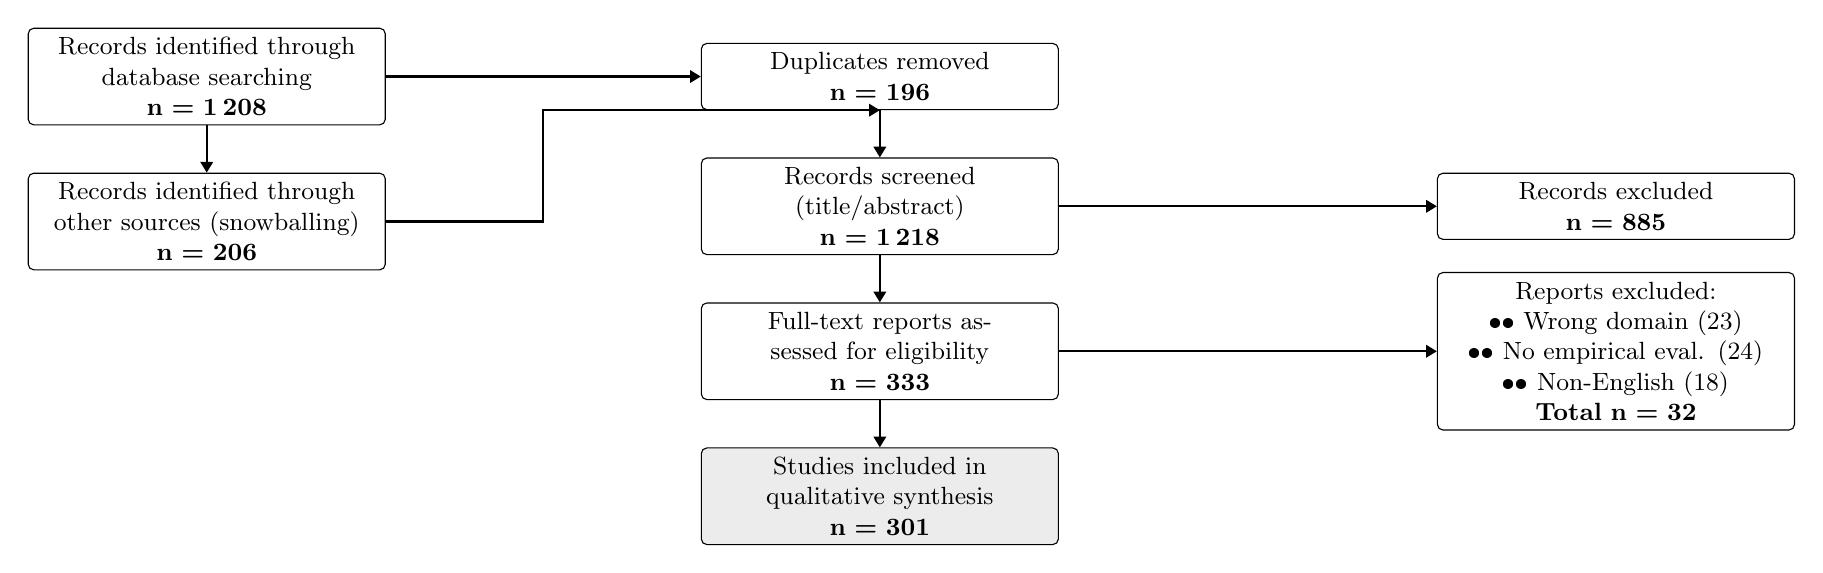
\begin{tikzpicture}[
    node distance = 6mm and 10mm,
    process/.style = {rectangle, draw, text width=4.3cm, align=center,
                      font=\small, rounded corners=2pt},
    arrow/.style   = {-{Triangle[scale=0.8]}, thick},
  ]
  % Identification
  \node[process] (id1) {Records identified through database searching \\ \textbf{n = 1\,208}};
  \node[below=of id1,process] (id2) {Records identified through other sources (snowballing) \\ \textbf{n = 206}};
  \draw[arrow] (id1.south) -- (id2.north);

  % Deduplication
  \node[right=4cm of id1,process] (de) {Duplicates removed \\ \textbf{n = 196}};
  \draw[arrow] (id1.east) -- (de.west);
  \draw[arrow] (id2.east) -- ++(0:2.0cm) |- (de.south);

  \node[below=of de,process] (screen) {Records screened (title/abstract) \\ \textbf{n = 1\,218}};
  \draw[arrow] (de.south) -- (screen.north);

  \node[right=4.8cm of screen,process] (excl) {Records excluded \\ \textbf{n = 885}};
  \draw[arrow] (screen.east) -- (excl.west);

  % Eligibility
  \node[below=of screen,process] (elig) {Full-text reports assessed for eligibility \\ \textbf{n = 333}};
  \draw[arrow] (screen.south) -- (elig.north);

  \node[right=4.8cm of elig,process] (excl2) {Reports excluded: \\•• Wrong domain (23) \\•• No empirical eval. (24) \\•• Non-English (18) \\ \textbf{Total n = 32}};
  \draw[arrow] (elig.east) -- (excl2.west);

  % Included
  \node[below=of elig,process,fill=gray!15] (incl) {Studies included in qualitative synthesis \\ \textbf{n = 301}};
  \draw[arrow] (elig.south) -- (incl.north);
\end{tikzpicture}}
\caption{PRISMA 2020 flow diagram for study selection (search cut-off 11 August 2025).}
\label{fig:prisma}
\end{figure*}
%-----------------------------------------------------------------------%


%--------------------  thematic distribution table --------------------%
\begin{table}[htbp]
  \centering
  \caption{Distribution of the 301 included studies by primary contribution.}
  \label{tab:taskdist}
  \begin{tabular}{@{}p{5.5cm}rp{6cm}@{}}
    \toprule
    \textbf{Category} & \textbf{\# Papers} & \textbf{Representative citations}\\
    \midrule
    Formal theorem proving           & 45 & \cite{xin2024deepseek,wu2022autoformalization,first2023baldur,anonymous2025deeptheorem,chen2025seedproverdeepbroadreasoning,shen2025realprover,zhou2025delta,wang2025letsreasonformally,poesia2024}\\
    Mathematical word-problem solving& 45 & \cite{wei2022chain,li2024gsmplus,gao2022pal,anonymous2025jtmath,anonymous2025cama,anonymous2025advancingmultistep,ariyarathne2025elementarymwp,yu-etal-2025-chain,liang2023let,guan2025rstar,zhong2024achieving,feng2024bstep,ye2024physics,deng2023,chen2024a,yang2023b,feng2024}\\
    Dataset / benchmark creation     & 75 & \cite{huang2024mustard,yang2024mathbench,tang2024mathscale,anonymous2025olympiadmath,anonymous2025benchmarkmathcreativity,anonymous2025reliablemath,anonymous2025polymatheval,anonymous2025llmthinkbench,perez2025ai4mathnativespanishbenchmark,zhang2024mathodyssey,anonymous2025varmath,yu2025formalmath,zhang2025realmath,balunovic2025matharena,chernyshev-etal-2025-u,depaiva2025mathnli,anonymous2025enigmata,he2024bolympiadbench,li2024cnuminamath,toshniwal2024aopenmathinstruct2,toshniwal2024bopenmathinstruct1,paster2024openwebmath,wei2023cmath,liu2023augmenting,huang2024key,fang2024,kurtic2024,mao2024,mirzadeh2024,zeng2024,han2024,liu2024b,liang2024c,lu2024b,chernyshev2024}\\
    Neuro-symbolic integration       & 18 & \cite{jackson2024neurosymbolic,romera2024mathematical,chen2024enhancingmathematicalreasoningllms,liang2025imo}\\
    Auto-formalisation               & 15 & \cite{wu2022autoformalization,murphy2024autoformalizing,wu2025stepfunformalizer,weng2025autoformalization_survey}\\
    Multimodal or diagrammatic math  & 25 & \cite{shi2024mathllava,wang2024mathv,wang2025mllm_math_survey,gao2023,shi2024,jia2024,gupta2024,kazemi2023,liang2023a,yang2024b,zhuang2024,zhang2024d,yan2024a,yan2025b}\\
    Conjecture / counter-example generation & 10
& \cite{chuharski2024conjecture,exploring2024conjecturing,
goldbach2024case,li2025countermath,countermath2024,
li2025countermath,agentichypothesis2025survey,anonymous2025leanconjecturer,anonymous2025leanconjecturer}\\
Ensemble / MoE reasoning               & 12
& \cite{kim2025every,deepseek2025r1,sparsity2024emnlp,internlm2024,internlm2024,ren2025sigma}\\
    Multilingual mathematical reasoning    & 6 & \cite{anonymous2025polymatheval,perez2025ai4mathnativespanishbenchmark,anonymous2025polymatheval,wei2023cmath}\\
    Evaluation and pitfalls                & 35 & \cite{anonymous2025evaluationmathsolving,anonymous2025evaluatingmathreasoning,anonymous2025beyondaccuracy,anonymous2025doesmath,anonymous2025whoreasons,anonymous2025canllmmath,anonymous2025wordsense,anonymous2025largescaleproofs,anonymous2025wordsense,anonymous2025evaluationmathsolving,anonymous2025evaluatingmathreasoning,anonymous2025canllmmath,anonymous2025doesmath,anonymous2025beyondaccuracy,anonymous2025whoreasons,anonymous2025largescaleemergence,calais-etal-2025-disentangling,liang2025quantifying,liu2025can,han2025can,shafayat2025can,anonymous2025canllmstrategic,guo2024learning,didolkar2024metacognitive,sprague2024ato,srivastava2024evaluating,guo2024a,mirzadeh2024,chen2025a}\\
    \bottomrule
  \end{tabular}
\end{table}
%-----------------------------------------------------------------------%

\section{Thematic Analysis}
\subsection{Formal Mathematics and Interactive Theorem Provers}
Formalized mathematics aims for machine‐checkable certainty, exceeding the rigor of traditional peer review. Its lineage spans from Hilbert and Russell's logistic programs to today’s expansive web-hosted libraries containing tens of thousands of verified theorems.  This section traces that evolution, surveys the ecosystems enabling large-scale formalization, and highlights landmark projects. It concludes with a review of how learning paradigms, both supervised and reinforcement, are being integrated into ITPs to accelerate proof development.

\subsubsection{Historical Evolution}\label{sec:history}
Early proof-checking systems like AUTOMATH and LCF demonstrated that substantial mathematics could be mechanized. These systems introduced the architecture of modern proof assistants, a small trusted kernel ensures soundness, while user level tactics perform automation \cite{paulson1986natural,paulson1988preliminary}.  Milestones such as McCune’s resolution of the Robbins conjecture \cite{mccune1997solution} and Paulson’s formalization of Gödel’s incompleteness theorems \cite{paulson2013godel} showcased the power of mechanized reasoning.  Studies like the \emph{de Bruijn factor} quantified the overhead of formalization \cite{wiedijk2012de}, while retrospectives charted the fields growth \cite{debruijn1994survey,harrison2014history}.

\subsubsection{Mature Libraries and Ecosystems}\label{sec:libraries}
The utility of an ITP depends not just on its kernel but on its surrounding library. Mizar's Mathematical Library sets the benchmark for breadth and editorial consistency \cite{bancerek2018role}. Isabelle's Sledgehammer tool bridges to external provers, automating low-level steps \cite{bohme2010sledgehammer}.  Lean’s \texttt{mathlib} exemplifies community-driven growth \cite{moura2021lean,mathlib4}, with Lean 4 introducing a re-engineered kernel and faster elaboration.  Tools like \texttt{Lean Dojo} expose millions of proof states for data mining \cite{yang2023leandojo}, while tutorials like the (\texttt{Lean Workbook}) lower the entry barrier \cite{ying2024leanworkbook,ying2024leanworkbook}.  LLMs are increasingly fine-tuned within these ecosystems, serving as proof-state predictors \cite{li2023aiformathematics,li2024leanreasoner} or assistants that retrieve documentation on demand \cite{song2024towards}. Innovations like \emph{Lean Copilot} and \emph{LeanProgress} embed LLMs directly into the IDE, reducing manual effort and guiding search \cite{huang2024leancopilot, huang2025leanprogress}. Other ecosystems, such as PVS via \texttt{MathPVS} \cite{saidi2023mathPVS}, show that no single library dominates all domains. Collectively, these infrastructures transform abstract kernels into dynamic mathematical databases growing at a journal-like pace \cite{massot2023mathematics}.  Experimental agents like \texttt{Theorem‐LLaMA} explore next-generation interfaces that unify code completion, premise search, and proof synthesis \cite{gu2024theoremllama}.

\subsubsection{Large-Scale Formalisation Projects}\label{sec:megaprojects}
Recent case studies demonstrate that modern ITPs can handle sophisticated mathematics. Isabelle has formalised Szemerédi’s Regularity Lemma \cite{edmonds2023formalising}, while Lean has encoded the theory of schemes \cite{buzzard2022schemes,bordg2022simple}, validating its capacity for category-heavy domains. The Liquid Tensor Experiment translated Scholze and Clausen’s condensed algebra into Lean, producing a corpus now mined by both symbolic and neural methods \cite{castelvecchi2021mathematicians,scholze2022half}. Other efforts include hyper-dual numbers for numerical analysis \cite{smola2021hyperdual}, diagram chasing in homological algebra \cite{zhang2024diagramformalization}, and verified Euclidean geometry \cite{murphy2024autoformalizing}. Benchmarks like \texttt{Formalising 25} and \texttt{AlphaGeometry} quantify proof reuse and tackle Olympiad-level problems \cite{buzzard2022formalising,trinh2024alphageometry}. Automated pipelines now translate informal implication graphs into Lean, hinting at partially self-driving formalization \cite{autoformalization2023,sinha2024wusmethod}.

\subsubsection{Learning with Interactive Theorem Provers}\label{sec:learning-itp}
The convergence of data-rich proof corpora and data-hungry neural models and has sparked a new research paradigm: training LLMs to operate \emph{within} ITPs. These efforts span both supervised and reinforcement learning, each offering distinct advantages for automating formal reasoning.  

\paragraph{Supervised learning.}  Public libraries and educational materials provide paired $(\text{goal},\text{proof})$ examples suitable for supervised learning.  Models like \texttt{ProofNet} predict Lean tactic sequences over undergraduate-level content, outperforming earlier baselines in both success rate and proof length \cite{azerbayev2023proofnet}.  Comparative studies reveal complementary strengths between LLMs and symbolic heuristics, motivating hybrid curricula that combine imitation learning with synthetic data augmentation \cite{johnson2024llmvsitp}.  Fine-grained vector embedding layers (FVEL) further enhance state representations, enabling deeper models without prohibitive compute costs \cite{song2024fvel}.

\paragraph{Reinforcement learning.}  Casting proof search as sequential decision-making allows agents to explore tactic space beyond human demonstrations.  \texttt{TacticZero} exemplifies imitation-free reinforcement learning, achieving non-trivial Lean benchmarks without reference proofs \cite{wu2021tacticzero}. \emph{RL-Theorem Prover}, fine-tunes a 0.5B-parameter model directly against Lean’s kernel rewards, outperforming supervised baselines on \textit{miniF2F} \cite{luo2025rltheorem}. The Draft–Sketch–Prove pipeline interleaves informal reasoning with interaction traces, shaping rewards across multiple temporal levels \cite{jiang2022draft}.  Decomposition techniques like \texttt{SubgoalXL} split large goals into auxiliary lemmas, reducing branching and improving off-policy credit assignment \cite{yang2023subgoalxl}.  Recent work decomposes entire proof development into hierarchical tasks, achieving state-of-the-art success rates on miniF2F and subsets of mathlib \cite{williams2024decomposing}. Cross-domain reinforcement learning has also shown promise in enhancing LLM reasoning capabilities \cite{cheng2025revisitingrl,anonymous2025revisitingrl}, while strategic reasoning studies highlight both limitations and opportunities for improvement \cite{park2025canllmstrategic,anonymous2025canllmstrategic}. A practical two-stage recipe combining supervised fine-tuning (SFT) and RL has been proposed for mathematical LLMs \cite{yoshihara2025twostage}. The Minimo agent introduces intrinsic motivation to simultaneously conjecture and prove, pushing towards autonomous mathematical discovery \cite{poesia2024}.

\paragraph{Hierarchical RL.}
  \textbf{DeepSeek-Prover-V2} achoeves
  88.9\,\% \emph{Pass@32} on \textit{miniF2F} by applying \emph{reinforcement-
  learning over recursively decomposed sub-goals}
  \cite{Ren2025DeepSeekV2}.  In parallel,
  \textbf{Lean-STaR} embeds a structured \emph{think $\rightarrow$ prove}
  loop, injecting informal reflection before each tactic and
  yielding an additional 2.9 percentage points on the same benchmark
  \cite{Lin2025LeanSTaR}.

Taken together, these learning paradigms offer a plausible route to reducing the human bottleneck in formalization.  Yet, they also raise fresh questions about robustness, verification of machine-generated proofs, and alignment of neural search strategies with the epistemic norms of mathematics—questions revisited in Sections~\ref{sec:evaluation}–\ref{sec:future}.

\subsection{LLMs for Mathematical Reasoning: Methodologies and Applications}
LLMs have transformed computer-aided mathematics by replacing handcrafted heuristics with statistical models capable of learning both syntax and informal semantics. This section synthesizes key methodological advances and their applications, focusing on proof generation, premise selection, verification, and integration with symbolic systems. 

\subsubsection{Generating Proof Steps}\label{sec:proof-steps}
Constructing complete proofs remains a central challenge. Recent approaches fall into several categories:   
\begin{itemize}
    \item \textbf{Retrieval-Augmented Provers}: Tools like \emph{LeanDojo} and \emph{Lean Copilot} combine LLMs with retrieval modules, outperforming GPT-4 on Lean benchmarks and reducing manual effort by up to 85\% \cite{yang2023leandojo, huang2024leancopilot}.
    \item \textbf{Foundation Models}: \emph{LLEMMA}, trained on ProofPile-2 and research papers, sets new open-weight performance on MATH without task-specific fine-tuning \cite{azerbayev2024llemma}.
\end{itemize}

\paragraph{Reinforcement learning for lemma invention.}
Dong~\emph{et al.} reward an agent not only for proving the target
goal but also for discovering \emph{useful auxiliary lemmas}; the scheme
improves Isabelle/HOL success from 40.8 \% to 45.5 \%
\cite{dong2024lemmaRL}. The result strengthens the case for hierarchical
RL as a complement to supervised imitation.

\paragraph{Step-by-step generation.}
Here, a model conditions on the current proof state and predicts the next tactic.  Early neural successors such as \texttt{NaturalProver} generated readable proofs for textbook geometry \cite{welleck2022naturalprover}.  The idea was refined by \texttt{LEGO-Prover}, whose modular skill library supports continual learning across domains \cite{xin2023lego,xin2023lego}.  Larger instruction-tuned variants, e.g.\  \emph{DeepSeek-Prover} \cite{xin2024deepseek} and its RL-enhanced v1.5 release that reaches 63.5 \% Pass@64 on \textit{miniF2F} \cite{xin2024deepseek15},  exploit hundreds of millions of Lean proof states mined automatically from \texttt{mathlib4}.  Empirical analyses reveal that transformer depth rather than parameter count best predicts success on hard combinatorics benchmarks \cite{yang2023steamroller}.  Verification‐aware decoders further improve reliability by discarding actions that violate kernel constraints in silico before any expensive tactic call \cite{cao2024verification}. Dual-correction orchestration in Lyra further cuts error propagation \cite{lee2024lyra}. Recent advances in synthetic verifiable proofs have further advanced LLM reasoning for theorem proving \cite{zhang2025deeptheorem,anonymous2025deeptheorem}, while deep and broad reasoning approaches like Seed-Prover enhance automated theorem proving capabilities \cite{chen2025seedproverdeepbroadreasoning}. Methods like Delta decompose formal math problems by decomposition and iterative reflection \cite{zhou2025delta}. Chain-of-Reasoning approaches aim for unified mathematical reasoning via multi-paradigm perspectives \cite{yu-etal-2025-chain}. SIGMA refines LLM reasoning via sibling-guided Monte Carlo augmentation \cite{ren2025sigma}. DeepCritic uses deliberate critique with LLMs \cite{yang2025deepcritic}. Twisted Sequential Monte Carlo (TSMC) has been proposed for step-by-step reasoning in math problems, refining estimates of correct reasoning paths \cite{feng2024}. Masked Thought introduces a simple masking strategy for partial reasoning steps to improve learning \cite{chen2024a}.

\paragraph{Whole-proof synthesis.}
One-shot generation sacrifices fine-grained control for global coherence.  \texttt{Baldur} demonstrated that GPT-4–class models can emit Lean proofs thousands of tokens long \cite{first2023baldur}.  Subsequent systems couple beam search with neural self-refinement, pruning globally inconsistent candidates during reranking \cite{smith2024linc}.  The Mathematical Divide and Conquer technique reverses the process: a model first proposes an abstract proof plan, then recursively realizes subgoals, achieving state-of-the-art scores on the miniF2F benchmark \cite{srivastava2024mathdivide}.  For Coq, dataset augmentation via automatically generated counterexamples proved critical for maintaining consistency in long outputs \cite{florath2024enhancing}.

\paragraph{Proof repair and self-verification.}
Even the best LLM occasionally hallucinates or omits a justification.  Self-consistency sampling detects such pathologies by comparing independently generated traces \cite{lewkowycz2022solving,lewkowycz2023donttrustverify}.  Luo et al.\ show that coupling this with symbolic re-execution inside Lean eliminates $>75\%$ of incorrect steps without manual intervention \cite{gupta2024saas}.  Complementary neuro-symbolic pipelines translate a failed proof back into natural language, localize the fault, and propose an amended tactic sequence \cite{jiang2023automated,jackson2024neurosymbolic}.  Large‐scale experiments on the MUSTARD corpus confirm that automatic repair more than doubles success rates when allowed a modest time budget \cite{huang2024mustard}.  Finally, \texttt{MathDivide} pairs every generated lemma with a machine-verifiable certificate whose validity can be checked to guarantee downstream soundness \cite{romera2024mathematical}. Safe enhances mathematical reasoning via retrospective step-aware formal verification \cite{liu-etal-2025-safe}. A self-consistency-based hallucination detection method enhances reasoning with structured checks \cite{liu2025}.

\subsubsection{Finding Useful Premises}\label{sec:premise}
Premise selection is often harder than proving subgoals.  Retrieval-augmented Lean agents embed definitions and goals in a shared metric space, achieving recall@50 above 90\,\% on large libraries like \texttt{mathlib4} \cite{yang2023leandojo}.  Generative models complement retrieval by inventing bridging lemmas absent from the library; DeepSeek-Prover does so implicitly through speculative reasoning \cite{xin2024deepseek}.  Hybrid systems now interleave both modes, dynamically deciding whether to call the retriever or the generator based on entropy over the proof state.  Dedicated premise-guidance pipelines such as the AITP Formal Premise Selection system couple a contrastively trained retriever with a proof-state-conditioned language model, raising Isabelle success rates while querying over 100K lemmas \cite{tworkowski-2022-formal-premise}. REAL-Prover uses a retrieval-augmented Lean prover for mathematical reasoning \cite{shen2025realprover}.

\subsubsection{Solving Math Word Problems}\label{sec:mwp}
Math word problems (MWPs) test an LLM’s ability to connect natural-language narratives with symbolic manipulation.  

\paragraph{Chain-of-thought prompting.}
Chain-of-thought prompting significantly improves performance on multi-step reasoning tasks.
Explicit reasoning traces markedly boost accuracy on GSM8K-style tasks \cite{wei2022chain}.  Least-to-most prompting further decomposes competition-level problems into ordered subgoals, reducing search entropy and improving success rates on GSM8K, SVAMP, and MATH \cite{zhou-2023-least}.  Self-improvement pipelines such as STaR curate new rationales from their own mistakes to bootstrap stronger verifiers without requiring additional human labels \cite{zelikman-2022-star}.  Distillation-oriented studies aim to keep these skills in compact students: Teaching Small Language Models to Reason transfers chain-of-thought supervision to 1–7B parameter models, while targeted skill injection preserves arithmetic competence during continued training \cite{magister-2023-teaching,sharma-2022-skill-injection}.  Interactive multi-round tutoring strategies further tailor demonstrations and self-reflection prompts to a student's weaknesses, facilitating reasoning transfer from proprietary teachers without exposing weights \cite{wang-2023-tailored-learning}.  Algorithmic prompting explicitly composes low-level skills so that models generalize beyond surface statistics to parity, addition, and mixed arithmetic routines \cite{zhou-2022-teaching-algorithmic}.  Cooperative reasoning frameworks such as CoRe pair a generator with multiple verifiers to supervise intermediate steps, yielding sizeable gains on GSM8K, SVAMP, and Math23K without resorting to massive models \cite{zhu-2023-core}.  TabMWP extends evaluation to semi-structured contexts with aligned tables and images \cite{lu-2022-tabmwp}, while PromptPG learns to select in-context exemplars for those settings via policy gradients, stabilising GPT-3's accuracy under prompt variation \cite{lu-2023-dynamic-prompt}.  MathPrompter cross-checks algebraic expressions and Python functions generated under zero-shot CoT, improving MultiArith accuracy by over 13 points while providing confidence estimates \cite{imani-2023-mathprompter}.  MathCoder interleaves natural-language rationales with executable programs and their outputs, pushing open models beyond GPT-4 on the competition-level MATH benchmark \cite{wang-2023-mathcoder}.  Continued pretraining on mathematics-heavy corpora yields specialists such as \textsc{Llemma}, which pivot between formal proofs, code, and tool use without extra instruction tuning \cite{azerbayev-2024-llemma}.  Chain-of-thought prompting has likewise migrated to structured tables, where explicit evidence decomposition yields large gains in aggregation accuracy \cite{zheng-2023-tabular-cot}.  Backward reasoning templates such as Fill in the Blank encourage models to plan proofs from the desired conclusion, lifting performance on multi-step word problems \cite{deb-2024-backward-reasoning}.  Hybrid instruction pipelines such as \textsc{MAmmoTH} further blend teacher traces with synthetic curricula to build math generalists in the 7--30B parameter range \cite{yue-2023-mammoth}.  Tool-augmented prompting frameworks like ChatCoT interleave conversational reasoning with calculator and CAS calls, while plan-and-solve prompting, AlignedCoT, and multi-aspect feedback refine intermediate steps through structured critique and culturally-aligned demonstrations \cite{chen-2023-chatcot,wang-2023-plan-and-solve,yang-2024-alignedcot,nathani-2023-maf}.  Analysis of student model trajectories suggests that collapsing reasoning trees into simpler abstractions can substantially improve sample efficiency without sacrificing accuracy \cite{yan2023complexsimpleunravelingcognitive}.  Despite these advances, evidence suggests that most contemporary models still rely on semantic pattern matching rather than symbolic manipulation when making in-context inferences, highlighting the limits of current methods \cite{tang2023largelanguagemodelsincontext}.  Empirical audits also caution that naive query/response augmentation can stagnate or even degrade generalisation, motivating more principled data curation strategies \cite{zhang-2024-query-augmentation,li-2024-mugglemath}.  Outcome-supervised value models such as OVM guide decoding toward globally promising paths, while dynamic voting ensembles prioritise coherent sub-traces without brute-force sampling \cite{yu2024ovmoutcomesupervisedvaluemodels,xue-2023-dynamic-voting}.  Analyses of search trajectories reveal a strong first-step advantage and motivate more informative initial hints like HoPC and universal self-consistency routines to stabilise long chains \cite{jain2024firststepadvantageimportancestarting,lei2025hintpseudocodehopc,chen2023universalselfconsistencylargelanguage}.  Independent robustness audits measure hallucination rates under adversarial perturbations, providing quantitative targets for future verification systems \cite{qian-2024-hallucination-eval}.  Structured supervision with relational abstractions compresses intermediate states into reusable schemas and boosts solver accuracy across algorithmic benchmarks \cite{nam-2022-relational-abstractions}, while the Memory-Interactive Learning Engine couples symbolic scratchpads with persistent external memory to improve robustness on Math23K \cite{wu-2022-mile}.  Curriculum-based training further strengthens generalisation: staged example selection for semi-structured prompts and small transformer curricula both transfer to held-out compositions and harder regimes \cite{nam-2022-ood-curriculum,nam-2022-ood-transformers}. Monte-Carlo tree search guided by learned energy functions further improves accuracy without additional fine-tuning by exploring diverse solution paths \cite{xu-2023-no-train}.  MetaMath bootstraps new question-answer pairs from high-performing base models, yielding 395K synthetic problems that significantly enhance downstream instruction tuning \cite{yu-2024-metamath}. Markup languages such as LPML structure prompts into declarative stages that reduce cascading errors, while targeted prompt interventions control algebraic hallucinations across equational reasoning benchmarks \cite{yamauchi-2023-lpml,meadows-2025-prompt-interventions}.  Curriculum-aware fine-tuning recipes further close the gap between pass@1 and pass@k performance on GSM8K and MATH by combining rejection sampling with lightweight preference optimization \cite{liu-2023-improving-finetune}.  When evaluated on the large-scale \texttt{GSM-Plus} benchmark, instruction-fine-tuned Gemini 1.5 Pro achieves $90.3\,\%$ but only if reasoning chains are retained during inference \cite{li2024gsmplus}. WizardMath fine-tunes Llama-2 with reinforced Evol-Instruct, raising GSM-Plus accuracy to 92\% \cite{luo2025wizardmath}.  AceMath pairs two-stage supervised fine-tuning with a mathematically
calibrated reward model and pushes state-of-the-art accuracy across
\textsc{GSM-Plus}, \textsc{FrontierMath} and \textsc{MathBench}, overtaking GPT-4o and
Qwen2.5-Math by 5–9 pp~\citep{liu2024acemath}. Multi-stage frameworks like JT-Math further advance mathematical reasoning capabilities \cite{anonymous2025jtmath,anonymous2025jtmath}, while methods like CAMA \cite{anonymous2025cama,anonymous2025cama} and multi-layered self-reflection with auto-prompting \cite{anonymous2025advancingmultistep,anonymous2025advancingmultistep} enhance multi-step reasoning. PromptCoT synthesizes Olympiad-level problems for mathematical reasoning \cite{zhao-etal-2025-promptcot}. Deeply Understanding the Problems (DUP) improves LLMs' math word problem-solving by extracting key information for better reasoning, achieving >97\% on GSM8K \cite{zhong2024achieving}. rStar-Math enables small LLMs to master math reasoning through self-evolved deep thinking \cite{guan2025rstar}. A study on Chain-of-Thought (CoT) shows it primarily benefits math and logic tasks, with limited gains elsewhere \cite{sprague2024a to}. Metacognitive capabilities allow LLMs to assess their own problem-solving processes \cite{didolkar2024metacognitive}. Learning from mistakes on grade-school math problems enhances model performance through error-correction data in pretraining \cite{ye2024physics}. A unified view of answer calibration improves multi-step reasoning in MWPs \cite{deng2023}. Masking partial reasoning steps enhances learning for MWPs \cite{chen2024a}. TSMC provides step-by-step reasoning for MWPs via twisted sequential Monte Carlo \cite{feng2024}. GPT can solve MWPs without a calculator \cite{yang2023b}.

\paragraph{Program-of-thought prompting.}
\texttt{Program-Aided Language} (PAL) compels the models to generate executable code, reducing arithmetic errors \cite{chen2022program,gao2022pal}.  The same paradigm underpins \texttt{MuggleMath}, which augments the interpreter with SymPy subroutines to solve math problems with precision \cite{li2024mugglemath}.
Earlier work further shows that program-synthesis agents can reach human-level performance on university mathematics exams when paired with few-shot prompting and step-by-step synthesis \cite{drori-2022-program-synthesis}.

\paragraph{Tool integration.}
LLMs increasingly interface with external tools such as CAS engines, theorem proves, and numerical solvers to enhance robustness.  A single agent might call Wolfram Alpha for integrals, Lean for algebra facts, and a numerical optimiser for floating-point checks, achieving robustness on the MATH benchmark’s geometry track \cite{frieder2023mathematical}. ToRA integrates tools for mathematical problem solving \cite{gou2023}.  Interleaf prompting alternates natural reasoning with symbolic tool calls, delivering gains even without extra gradient updates \cite{chen-2023-interleaf}.  Logic-LM follows a similar philosophy, translating problems into first-order logic and delegating inference to a symbolic solver with iterative self-refinement \cite{pan-2023-logiclm}.  Meta-reasoning strategies increasingly arbitrate between natural-language chains and programmatic solvers, selecting the better trajectory on a per-problem basis to cut inference cost while boosting accuracy \cite{zhao-2023-auto-model-selection}.  Deliberate search frameworks such as Tree-of-Thoughts and retrieval-augmented multi-modal CoT harness lookahead, backtracking, and external memory to navigate long-horizon puzzles far more effectively than greedy decoding \cite{yao-2023-tree-of-thoughts,liu-2024-ramcot}.  Tool-interactive critiquing frameworks like CRITIC further automate self-correction by invoking calculators, search engines, and unit checkers before rewriting outputs \cite{gou2024criticlargelanguagemodels}.  ReWOO goes a step further by decoupling observation gathering from reasoning, allowing planners to operate on cached tool results for substantial speed-ups without sacrificing accuracy \cite{xu2023rewoodecouplingreasoningobservations}.  Studies of intrinsic critique ability explore when models can propose their own revisions without heavy prompting, offering lighter-weight safety scaffolds \cite{luo2023critiqueabilitylargelanguage}.  A complementary evaluation suite stresses computation-intensive tool use, benchmarking both plug-and-play retrieval strategies and learned controllers across symbolic algebra packages and custom Python sandboxes \cite{zhang-2023-tool-aug}.

\subsubsection{Autoformalization}\label{sec:autoformal}
Autoformalization bridges informal exposition and formal proof languages, lowering barriers to formal mathematics.

\paragraph{Sentence-level translation.}
Early attempts framed the task as semantic parsing \cite{wang2018first}.  Modern LLMs achieve one-shot translation for competition problems in Isabelle/HOL with accuracy exceeding 70\,\% \cite{wu2022autoformalization}.  The \texttt{AutoFormal-Functional} system extends the pipeline to Lean 4, preserving functional extensionality and universe levels automatically \cite{buali2024towards}. A complementary filter that scores candidates by symbolic equivalence and semantic fidelity further boosts translation accuracy \cite{li2024symbolicautoformal}.

\paragraph{Document-level workflows.}
\texttt{TheoremLlama} repurposed a 70-billion-parameter decoder as a Lean expert via multi-stage instruction tuning and synthetic bootstrapping \cite{gu2024theoremllama}.  Yang et al.\ push further, demonstrating mixed-modality translation that jointly processes diagrams and text for Euclidean geometry \cite{wu2022autoformalization,murphy2024autoformalizing}. Consistent Autoformalization uses retrieval-augmented correction loops to maintain library style \cite{zhang2024consistentautoformal}, and the new \textit{Def$^{+}$} datasets show that definition formalization remains especially challenging \cite{zhang2025definitions}. 	exttt{math-PVS} maps scientific prose into the Prototype Verification System, coupling bibliographic parsing with ontology alignment to seed machine-checkable theories for downstream automation \cite{saidi-2023-mathpvs}. StepFun-Formalizer unlocks autoformalization potential through knowledge-reasoning fusion \cite{wu2025stepfunformalizer}.

\paragraph{Visual-diagram reasoning.} Diagram-centric agents such as \emph{Geo-LLaVA} tackle 3-D geometry with retrieval-augmented VLMs \cite{gao2024geollava}, while \emph{Math-PUMA} aligns textual and visual embeddings in a three-stage curriculum, closing the modality gap observed on \textsc{MathVerse} \cite{zhuang2025mathpuma}.

\subsubsection{Datasets and Benchmarks}\label{sec:datasets}
Rigorous evaluation demands standardised corpora.

\begin{itemize}
    \item \textbf{\texttt{MUSTARD}} offers 6.7 M Lean proof steps with failure annotations for repair studies \cite{huang2024mustard}. 
    \item \textbf{\textsc{FormAI}} links formal-verification proofs with software-security use-cases \cite{johnson2024formai}.
    \item \textbf{\texttt{MathBench}} unifies 20 prior natural-language benchmarks under a common JSON schema, enabling fine-grained skill diagnostics \cite{yang2024mathbench}.  
    \item \textbf{\texttt{MathOdyssey}} introduces progressively harder curricula spanning arithmetic to abstract algebra \cite{zhang2024mathodyssey,zhang2024mathodyssey}.  
    \item \textbf{\texttt{GSM-Plus}} doubles GSM8K’s size and injects adversarial distractions to test chain robustness \cite{li2024gsmplus}.  
    \item \textbf{\texttt{MetaMath-QA}} focuses on formal statements paired with informal explanations, bridging Section \ref{sec:autoformal} and MWPs \cite{metamath2024,yu2024metamath}.
    \item \textbf{\texttt{LongerMath}} stresses long-context reasoning \cite{liu2024llmslongermath}.
    \item \textbf{\texttt{OpenMathReasoning}} (540 K Olympiad–level problems + 3.2 M long CoT + 1.7 M tool-augmented traces) fuels the 2025 AIMO-2 champion model \cite{Moshkov2025OpenMath}.
    \item \textbf{\textsc{FrontierMath}} – 300 unpublished research-level problems; current SOTA $<2$ \% \cite{Glazer2025FrontierMath}.
    \item \textbf{\texttt{miniCTX}} pairs 2.1 K Lean theorems with up to 60 k-token project files, isolating long-context dependency \cite{Hu2025miniCTX}.
    \item \textbf{\texttt{UGMathBench}} offers 5 062 under-grad problems across 16 subjects plus two new evaluation metrics (\textit{Effective-Accuracy}, \textit{Reasoning-Gap}) \cite{Xu2025UGMathBench}.
    \item \textbf{\textsc{MathVerse}} evaluates visual-text alignment across 2.6 K diagram-based problems rendered in six modality variants \cite{zhang2024mathverse}.
    \item \textbf{OlympiadMath} provides an Olympiad-level math benchmark for LLMs \cite{anonymous2025olympiadmath,anonymous2025olympiadmath}.
    \item \textbf{VarMath} probes true mathematical reasoning in LLMs \cite{anonymous2025varmath,anonymous2025varmath}.
    \item \textbf{LLMThinkBench} evaluates basic math reasoning and overthinking in LLMs \cite{anonymous2025llmthinkbench,anonymous2025llmthinkbench}.
    \item \textbf{AI4Math} offers a native Spanish benchmark for university-level mathematical reasoning \cite{perez2025ai4mathnativespanishbenchmark}.
    \item \textbf{PolyMathEval} assesses mathematical reasoning in multilingual contexts \cite{anonymous2025polymatheval,anonymous2025polymatheval}.
    \item \textbf{ReliableMath} benchmarks reliable mathematical reasoning on LLMs \cite{anonymous2025reliablemath,anonymous2025reliablemath}.
    \item \textbf{MathCreativity} evaluates mathematical creativity in LLMs \cite{anonymous2025benchmarkmathcreativity,anonymous2025benchmarkmathcreativity}.
    \item \textbf{FormalMATH} benchmarks formal mathematical reasoning of LLMs \cite{yu2025formalmath}.
    \item \textbf{RealMath} provides a continuous benchmark for research-level mathematics \cite{zhang2025realmath}.
    \item \textbf{MathArena} evaluates LLMs on uncontaminated math competitions \cite{balunovic2025matharena}.
    \item \textbf{U-MATH} is a university-level benchmark for mathematical skills \cite{chernyshev-etal-2025-u,depaiva2025mathnli,anonymous2025enigmata,he2024bolympiadbench,li2024c numinamath,toshniwal2024a openmathinstruct2,toshniwal2024b openmathinstruct1,paster2024openwebmath,wei2023cmath,liu2023augmenting,huang2024key,fang2024,kurtic2024,mao2024,mirzadeh2024,zeng2024,han2024,liu2024b,liang2024c,lu2024b,chernyshev2024,lu2024c}.
    \item \textbf{Math NLI} focuses on natural language inference in math \cite{depaiva2025mathnli}.
    \item \textbf{Enigmata} scales logical reasoning with synthetic verifiable puzzles \cite{anonymous2025enigmata}.
    \item \textbf{OlympiadBench} is a challenging benchmark for promoting AGI with Olympiad-level bilingual multimodal scientific problems \cite{he2024bolympiadbench}.
    \item \textbf{NuminaMath} is the largest public dataset in AI4Maths with 860k pairs of competition math problems and solutions \cite{li2024c numinamath}.
    \item \textbf{OpenMathInstruct-2} accelerates AI for math with massive open-source instruction data, consisting of 14M question-solution pairs \cite{toshniwal2024a openmathinstruct2}.
    \item \textbf{OpenMathInstruct-1} is a 1.8 million math instruction tuning dataset \cite{toshniwal2024b openmathinstruct1}.
    \item \textbf{OpenWebMath} is an open dataset of high-quality mathematical web text \cite{paster2024openwebmath}.
    \item \textbf{CMATH} tests if language models can pass Chinese elementary school math tests \cite{wei2023cmath}.
    \item \textbf{KPMath} is an extensive synthetic dataset for mathematical reasoning generated via key-point-driven data synthesis \cite{huang2024key}.
    \item \textbf{MathOdyssey} benchmarks mathematical problem-solving skills using Odyssey math data \cite{fang2024}.
    \item \textbf{Mathador-LM} is a dynamic benchmark for mathematical reasoning on LLMs \cite{kurtic2024}.
    \item \textbf{CHAMP} is a competition-level dataset for fine-grained analyses of LLMs' mathematical reasoning capabilities \cite{mao2024}.
    \item \textbf{GSM-Symbolic} understands limitations of mathematical reasoning in LLMs \cite{mirzadeh2024}.
    \item \textbf{Skywork-Math} provides data scaling laws for mathematical reasoning \cite{zeng2024}.
    \item \textbf{InfiMM-WebMath-40B} advances multimodal pre-training for enhanced mathematical reasoning \cite{han2024}.
    \item \textbf{MathBench} evaluates theory and application proficiency of LLMs with a hierarchical mathematics benchmark \cite{liu2024b}.
    \item \textbf{MathChat} benchmarks mathematical reasoning and instruction following in multi-turn interactions \cite{liang2024c}.
    \item \textbf{InfiMM-Eval} targets open-ended multi-modal reasoning with tasks that mix chart reading, algebra, and textual inference \cite{han2023infimmevalcomplexopenendedreasoning}.
    \item \textbf{MathGenie} generates synthetic data with question back-translation for enhancing mathematical reasoning \cite{lu2024b}.
    \item \textbf{U-MATH} is a university-level benchmark for evaluating mathematical skills in LLMs \cite{chernyshev2024}.
\end{itemize}

\subsubsection{Neuro-symbolic Integration}\label{sec:neurosym}
Purely neural models often struggle with long-range logical dependencies, while symbolic engines lack adaptive heuristics. Hybrid neuro-symbolic systems aim to combine their strengths.

Jackson et al.\ embed Lean proof states and tactic sequences into graph neural networks that a transformer consults when predicting actions, yielding a 12-point gain on miniF2F \cite{jackson2024neurosymbolic}.  Gupta et al.\ frame Lean as a software-as-a-service endpoint, allowing the language model to query a verifier during decoding without retraining \cite{gupta2024saas}.  Romera-Paredes et al.\ propose Mathematical LINC, where a symbolic controller decides when to switch between depth-first neural search and breadth-first SAT solving, reducing average proof length by 22 \% \cite{romera2024mathematical}. Enhancing mathematical reasoning via ontology-guided knowledge graphs further advances neuro-symbolic approaches \cite{chen2024enhancingmathematicalreasoningllms}. Approaches like decoupled reasoning and proving aim to solve more challenging IMO problems \cite{liang2025imo}. Natural-formal hybrid reasoning enhances LLM's math capability \cite{wang2025letsreasonformally}.

\paragraph{Conjecture formulation \& counter-example discovery.}
\citet{chuharski2024mining} introduce a \emph{generate–prune} workflow
in which a general-purpose LLM proposes candidate statements in
finite-group theory and then tries to \emph{disprove its own outputs}.
Self-generated counterexamples prune 78 \% of false conjectures, and
83\% % of the survivors hold across all test groups—an absolute
46 pp gain over likelihood-only filtering. Independently, a
neuro-symbolic CEGIS pipeline couples an LLM with a SAT solver and
refutes 71\% % of false Lean conjectures in under ten
seconds~\cite{jha2023neurosymbolic}. These approaches highlight the importance of tight iteration between generation and verification in open ended mathematical discovery. 


\subsubsection{Agents and Tooling}\label{sec:agents}
LLM agents wrap core capabilities into interactive interfaces for end-users, enabling pratical deployment in mathematical workflows. Foundation-models customised for mathematics—e.g.\ QwenMath \cite{yang2024qwenmath}, InternLM-Math \cite{ying2024 b internlm}—are now exposed via agent shells.

\begin{itemize}
    \item \textbf{MathAgent} orchestrates a multi-expert planner
(retrieval -> tactic -> verifier) able to \emph{both} construct proofs and
suggest “next-step” conjectures, yielding a 12-point gain on
algebraic-geometry benchmarks over single-agent
baselines~\cite{yan2025mathagent}.    
    \item \textbf{\texttt{TORA}} orchestrates multiple specialised LLMs—one for retrieval, one for tactic prediction, one for verification—to achieve fault tolerance on noisy prompts \cite{gou2024tora}.  
    \item \textbf{\texttt{MathSensei}} serves as an adaptive tutoring system, synthesising hints and partial proofs tailored to a student’s misconceptions \cite{sun2024mathsensei}.  
    \item \textbf{AIMO-2 Progress Prize} (Apr 2025) showed that
    open-weight models, trained principally on
    \texttt{OpenMathReasoning}, can now solve \textbf{34 / 50} fresh
    Olympiad problems under strict compute limits
    \cite{Moshkov2025OpenMath}.
    \item \textbf{\texttt{MathAgents}} exposes a planning-execution loop that decomposes research-level conjectures into verifiable subtasks \cite{jones2024mathagents}. 
    \item \textbf{MACM} utilizes a multi-agent system for condition mining in solving complex mathematical problems \cite{lei2024}.
    \item \textbf{MathAgent} leverages a mixture-of-math-agent framework for real-world multimodal mathematical error detection \cite{yan2025b}.
\end{itemize}

\paragraph{Open computer–algebra back-ends.}
Most neuro-symbolic agents currently rely on proof assistants or general-purpose CAS APs. However, advanced tasks in algebraic geometry and number theory often require specialized algebraic tools.
\textsc{OSCAR} \cite{bosma2021oscar} is a modern open-source system that integrates Gröbner–basis computation, ideal arithmetic, polyhedral
geometry, and number-theoretic routines behind a programmatic interface.
Its JSON-RPC enables direct integration with LLM tool-calling pipelines, bridging high-level reasoning and low-level algebraic manipulations for tasks like variety analysis and dimension counting.

\paragraph{Collaborative multi-agent deliberation.}
While most frameworks rely on a single LLM for planning and verification, recent works show that explicit agent
\emph{collaboration} can significantly improve performance.
\citet{du2024collabgeo} coordinate four specialized GPT-4 agents
(\emph{Planner}, \emph{Solver}, \emph{Critic}, and \emph{Drawer}) that debate
interactively to solve synthetic-geometry construction problems.
The deliberation protocol improves task accuracy by up to
18\,percentage points over strong single-agent baselines, underscoring the
value of communication and cross-checking in complex spatial reasoning.
These results strengthen the case for MathScy’s proposed multi-agent design,
where distinct experts handle conjecture generation, proof search and
counter-example generation in a tightly coupled loop.

\subsubsection{Mixture-of-Experts and Ensemble-Reasoning Paradigms}
\label{sec:moe}

\textbf{Sparse MoE Transformers.}  
Models like \emph{Mixtral 8$\times$7B}
demonstrate that sparse-activated MoE layers can match or outperform larger dense models on multi-step reasoning tasks while running
$\sim\!6\times$ faster at inference
\citep{jiang2024mixtral}.%
\footnote{Mixtral’s licence (Apache 2.0) has already made it the default
“reference MoE” for multiple academic benchmarks.}
Though general purpose, Mixtral shows strong performance on GSM8K and MATH, suggesting the emergence of latent \emph{math-specialist} sub-experts.

\textbf{Domain-specialist MoE assembly.}  
\emph{Branch-Train-MiX} (Section \ref{sec:neurosym}) trains domain-specific
experts in parallel and later merges them into a single routed model.
A contemporaneous residual variant, \emph{S’MoRE}, pushes the same idea
into parameter-efficient fine-tuning by attaching low-rank residual experts
that are gated on-the-fly, eliminating catastrophic forgetting while
adding only a few percent of new parameters
\citep{zeng2025smore}.

\textbf{Ensemble-of-LLMs as a symbolic MoE.}  
A complementary line of work dispenses with joint training altogether
and instead composes multiple \emph{fully trained} LLMs via a symbolic
router.  \emph{Symbolic-MoE} profiles each candidate model’s skill set,
then selects a sparse subset of experts per query, fusing their answers
with a learned aggregator.  On AIME and MMLU-Pro it yields an
$8.1\%$ accuracy boost over the best single model while cutting runtime
by $44\%$ \citep{chen2025symbolicmoe}.

\textbf{Training-time opinion ensembles.}  
\emph{Mixture-of-Opinions (MoO)} draws chain-of-thought traces from
weaker peer models and feeds them to a stronger student during fine-tuning,
acting as a lightweight knowledge-distillation MoE.  The method adds
$\approx5$ absolute points on GSM8K and AQuA without increasing model
size \citep{chen2025mixtureopinions}.

\textbf{Prompt-level MoE.}  
The earlier \emph{Mixture-of-Reasoning-Experts (MoRE)} showed that
prompt-specialised experts (factual, multihop, math, commonsense) plus a
simple answer-selector already outperforms single-prompt baselines across
12 QA datasets, with especially large gains on math word problems
\citep{si2023more}.  Despite relying on a single underlying LLM, MoRE
validates the hypothesis that \emph{diverse reasoning paths} combined
with selective routing, it improves reliability.

\paragraph{Beyond sparse MoE layers.}
\emph{Mixture-of-Reasoning-Experts} partitions a single backbone into
prompt-specialized experts (math, factual, multihop, commonsense) and
uses answer agreement to boost reliability~\cite{si2023more}. A related
training-time ensemble, \emph{Mixture of Opinions}, distils reasoning
traces from weaker peer models into a stronger student, gaining
5 pp accuracy on GSM8K without adding parameters~\cite{chen2025moo}. The
most recent \emph{Symbolic-MoE} framework treats entire LLMs as routable
skills—algebra, geometry, topology, \emph{etc.}—and selects a sparse
subset per query, beating a single GPT-4 baseline on AIM-E while running
44 \% faster at inference~\cite{chen2025symbolicmoe}. Together, these
results indicate that \textbf{strategic specialization and routing may
trump further parametric scaling} for mathematical reasoning workloads.

\paragraph{Knowledge-distilled MoE.}
\citet{kim2025every} shows that careful expert-wise distillation (“Every
Expert Matters”) transfers a sparse MoE into a \emph{dense} student
while adding +5 pp GSM8K and +4 pp MATH—evidence that routing diversity
rather than raw parameter count drives math performance.

\paragraph{Large-scale sparse routing.}
\textsc{DeepSeek-R1} (671 B total / 37 B active) is the largest
open-weight MoE released so far. Reinforcement learning on 7.1 M Lean
traces lifts miniF2F \textit{Pass@32} by 9 pp over an equally-sized
dense baseline, with ablations pinpointing gate accuracy on long proofs
as the remaining bottleneck~\cite{deepseek2025r1}.

\paragraph{Inference-optimised MoE frameworks.}
The recent surge of \emph{serving-time} research has produced a parallel strand of work that complements the architectural and training-time methods already surveyed.  
\begin{itemize}
  \item \textbf{eMoE}~\cite{tairin2025emoe} predicts future token–expert routes and pre-loads only the experts that are likely to be used, trimming \mbox{$\sim$80\%} of GPU memory while cutting latency by up to 17\,\%.  
  \item \textbf{MoEShard}~\cite{balmau2025moeshard} achieves perfect load-balancing by \emph{tensor-sharding} every expert across GPUs, realizing up to $6.4\times$ faster time-to-first-token than DeepSpeed baselines.  
  \item \textbf{DeepSpeed-MoE / PR-MoE}~\cite{rajbhandari2022deepspeedmoe} delivers an end-to-end training–inference stack and introduces the \emph{Pyramid-Residual MoE}, a hybrid dense–sparse design that compresses model size by $3\times$ with negligible quality loss.  
  \item \textbf{Speculative-MoE (s-MoE)}~\cite{li2025speculativemoe} reduces cross-device communication via speculative token shuffling and expert pre-grouping, yielding up to 75 \% lower bandwidth and $2.4\times$ higher throughput.  
  \item \textbf{MoE-Gen}~\cite{xu2025moegen} targets single-GPU deployment: by batching at the \emph{module} (attention vs.\ expert) level, it realizes $8$–$31\times$ throughput gains over continuous-batching engines such as vLLM on Mixtral and DeepSeek models.  
\end{itemize}

\noindent
These systems demonstrate that \emph{routing and memory scheduling} can be as critical as model size or expert specialization for real-world efficiency.  We therefore categorize them as the emerging \emph{inference-optimized MoE} sub-family and flag them as a high-leverage target for future work on cost-effective mathematical LLMs.%

Collectively, these approaches indicate that the next leap in
mathematical reasoning may hinge less on brute-force model size and more
on \emph{strategic specialization}—either at the token level (sparse MoE
layers) or at the system level (ensemble routing).


\subsubsection{Conjecture formulation with large language models}
\label{subsec:conjLLM}
%=================================================================
Early evidence suggests that LLMs can function as \emph{creative aides}
for hypothesis generation when paired with rigorous validation
pipelines.

\paragraph{Generate–prune in algebra.}
Chuharski~\emph{et al.} prompt GPT-4–class models to invent candidate
group-theoretic statements, then automatically call \textsc{gap} to seek
counterexamples. Roughly one-third of the conjectures produced by the
model were \emph{non-trivial} and survived brute-force falsification,
illustrating that stochastic language models can surface viable
hypotheses for specialist review~\cite{chuharski2024conjecture}.

\paragraph{FunSearch: LLM-guided evolutionary discovery.}
DeepMind’s \emph{FunSearch} couples a pre-trained LLM with an
evolutionary search that retains only candidates improving a numeric
objective. Applied to the cap-set problem, the system produced new
constructions that beat the best published bounds, a result
later published in \emph{Nature}
\cite{romeraparedes2024funsearch}. The same framework found improved
heuristics for online bin-packing, underlining its generality.

\paragraph{Towards agentic hypothesis generation.}
A recent survey on “agentic” scientific discovery highlights LLM-driven
hypothesis generation across domains, with mathematics singled out as a
particularly promising test-bed
\cite{agentichypothesis2025survey}. Echoing Lakatos, the authors argue
for tight conjecture–refutation loops in which the LLM both proposes and
attempts to falsify its own ideas—an approach revisited in
Section~\ref{subsec:counterexamples}. Automatic generation of mathematical conjectures for theorem proving has been advanced through tools like LeanConjecturer \cite{anonymous2025leanconjecturer}.


\subsubsection{Counterexample finding and falsification}
\label{subsec:counterexamples}
%=================================================================
Whereas proof synthesis shows that a statement is \emph{true},
counterexample generation provides evidence of \emph{falsehood} and is
crucial for robust mathematical discovery.

\paragraph{Benchmarking the skill.}
\emph{CounterMATH} offers 1.2 k undergraduate-level statements whose
correct “solution’’ is a concrete counterexample; GPT-4 solves barely
14 \% out-of-the-box, revealing a gap in present-day
models~\cite{li2025countermath}. Fine-tuning on synthetic,
counterexample-rich data narrows—but does not close—that gap.

\paragraph{Counterexample-guided pruning.}
The \emph{LIPS} pipeline for Olympiad-level inequalities prompts an LLM
for algebraic transformations and instantly \emph{rejects} any step that
fails on a randomly sampled instantiation, using a CAS as oracle. This
self-debugging loop halves hallucination rates and delivers SOTA results
on 161 hard inequalities~\cite{li2025lips}. Similar LLM–solver hybrids
are appearing in geometry, combinatorics, and number theory.


\bigskip
Collectively, the methodologies surveyed in this section underline a trend toward interactive, verification-aware, and data-rich LLM frameworks.  Subsequent sections will interrogate how well these systems actually generalize, how fairly they are benchmarked, and what open challenges remain.

\subsubsection{Multimodal Mathematical Reasoning}\label{sec:multilingual}
Recent advancements have emphasized the importance of mathematical reasoning in non-English languages. Benchmarks such as PolyMathEval evaluate reasoning in multilingual contexts \cite{anonymous2025polymatheval,anonymous2025polymatheval}, while AI4Math provides a native Spanish dataset for university-level problems \cite{perez2025ai4mathnativespanishbenchmark}. These efforts reveal performance gaps in current LLMs and highlight the need for culturally diverse training data to ensure equitable access to AI-assisted mathematics. CMATH tests if models can pass Chinese elementary school math tests \cite{wei2023cmath}. Targeted adaptation strategies further show that bilingual fine-tuning and cross-lingual prompt augmentation can close more than half of the accuracy gap between English and low-resource languages on competition datasets \cite{chen-2024-multilingual-math}.  Purpose-built Chinese models such as Jiuzhang 2.0 couple symbolic tools with curriculum pre-training to reach competition-level accuracy across algebra, geometry, and word problems \cite{sun-2023-jiuzhang}.  Model-level interventions such as Olapa-MCoT pair alignment-aware fine-tuning with rejection sampling to lift Chinese contest accuracy by 36 percentage points while preserving English skills \cite{zhu-2023-olapa-mcot}.  Broader multilingual efforts like YAYI 2 and the CLEVA evaluation platform emphasise end-to-end pipelines for curating diverse corpora and testing Chinese-centric mathematical ability \cite{luo2023yayi2multilingualopensource,li2023clevachineselanguagemodels}.

The multimodal aspect is crucial for handling diagrams and visual elements in math. G-LLaVA solves geometric problems with multimodal LLMs \cite{gao2023}. Math-LLaVA bootstraps mathematical reasoning for MLLMs \cite{shi2024}. MatCha augments Pix2Struct pretraining with chart derendering and numerical reasoning objectives, boosting accuracy on PlotQA and ChartQA by nearly 20 points \cite{liu-2023-matcha}. MathVista aggregates 6.4K multimodal problems spanning diagrams, plots, and videos, offering standardized evaluation for visual mathematical reasoning across 28 tasks \cite{lu-2024-mathvista}. Describe-then-Reason improves multimodal mathematical reasoning through visual comprehension training \cite{jia2024}. PolyMath is a challenging multimodal mathematical reasoning benchmark \cite{gupta2024}. GeomVerse systematically evaluates large models for geometric reasoning \cite{kazemi2023}. MathGLM-Vision solves mathematical problems with multimodal LLMs \cite{yang2024b}. Math-PUMA progressively aligns multimodal data to enhance mathematical reasoning \cite{zhuang2024}. GeoEval benchmarks LLMs and multimodal models on geometry problem-solving \cite{zhang2024d}. ErrorRadar benchmarks complex mathematical reasoning of MLLMs via error detection \cite{yan2024a}. MathAgent leverages a mixture-of-math-agent framework for real-world multimodal mathematical error detection \cite{yan2025b}. UniMath is a foundational and multimodal mathematical reasoner \cite{liang2023a}.  Cross-model comparisons of GPT-4V and allied multimodal systems reveal persistent weaknesses in structured visual reasoning, motivating hybrid neuro-symbolic approaches \cite{singh2023assessinggpt4vstructuredreasoning}. InfiMM-WebMath-40B advances multimodal pre-training for enhanced mathematical reasoning \cite{han2024}.  UniMath unifies textual, diagrammatic, and symbolic inputs under a single encoder–decoder, delivering consistent gains across geometry, chart, and algebra benchmarks \cite{liang-2023-unimath}.  Domain-specific pilots extend these pipelines to geometric algebra, combining retrieval with fine-tuning to support advanced mathematical languages \cite{wang-2023-geometric-algebra}.

\subsection{Evaluation, Robustness, and Ethics}\label{sec:evaluation}
A dependable assessment regime is indispensable if LLM‐assisted mathematics is to mature from speculative prototypes into scientific infrastructure.  Recent surveys catalog mathematical language models alongside over sixty task-specific datasets, underscoring how evaluation design co-evolves with model capability \cite{liu-2025-math-lm-survey}.  The community has therefore converged on three intertwined research thrusts: (i) constructing benchmark corpora that probe diverse skills under controlled conditions, (ii) analyzing robustness and failure modes—including hallucination, arithmetic drift, and strategic blindness—and (iii) interrogating the ethical implications of deploying stochastic reasoners in domains that prize certainty.

\subsubsection{Benchmark Corpora and Metrics}\label{sec:benchmarks}
Comprehensive datasets provide the substrate on which progress is measured.  Early work leveraged general reasoning suites, but their coverage and granularity proved insufficient for higher mathematics.  Contemporary resources instead specialize along skill axes, difficulty levels, or formal–informal boundaries.

\begin{itemize}
    \item \textbf{\textsc{MathBench}} unifies 20 legacy benchmarks under a hierarchical taxonomy covering arithmetic, algebra, geometry, and proof synthesis, standardizing input–output formats for reproducibility \cite{yang2024mathbench,mathbench2024}.  
    \item \textbf{MultiTaskMath} widens the scope further by injecting functional analysis, combinatorics, and topology problems; its deliberate multi‐distribution split exposes overfitting to a single curriculum \cite{bang2023multitask}.  
    \item \textbf{GSM‐Plus} doubles the canonical GSM8K set and appends adversarial distractions to stress‐test chain‐of‐thought robustness \cite{li2024gsmplus}.  Parallel efforts such as \textbf{XWinMath} extend cross‐lingual coverage to eight major languages \cite{li2024xwinmath}.  
    \item \textbf{Lila} unifies 20+ public math benchmarks under consistent splits and metadata, enabling apples-to-apples progress tracking across arithmetic, competition, and proof-style evaluations \cite{mishra-2023-lila}.  
    \item Domain‐specific suites include \textbf{OlympiadBench} for synthetic geometry \cite{he2024bolympiadbench}, \textbf{InfIMM} for information theory \cite{han2024infimm}, and \textbf{MATHV} for graduate‐level analysis and topology \cite{wang2024mathv}.  \n    \item \textbf{TRIGO} focuses on reducing formal proofs into human-like explanations, evaluating proof compression for generative models \cite{xiong2023trigobenchmarkingformalmathematical}.\n    \item \textbf{VerityMath} couples unit-consistency checks with self-verification scripts to probe numerical reliability \cite{han2024veritymathadvancingmathematicalreasoning}.
    \item Finance-oriented evaluations such as \textbf{FinanceMath} examine knowledge-intensive quantitative reasoning across analyst reports and financial statements \cite{zhao-2024-financemath}.  
    \item On the formal side, \textbf{BranchTrainMix} mixes verified Lean states with curriculum‐aware decoys to gauge premise selection difficulty \cite{wang2024branchtrainmix}, while \textbf{DeepSeekMath} captures 7.1M labelled Lean steps for large‐scale pre-training \cite{shao2024deepseekmath}.  
    \item Evaluation harnesses such as \textbf{MarO‐Eval} wrap these corpora in dockerised pipelines, enabling byte‐for‐byte reproducibility across hardware stacks \cite{zhang2024marioeval}.  
    \item \textbf{\textsc{MathVerse}} (visual maths) probes whether multimodal LLMs truly exploit diagrams \cite{zhang2024mathverse}.
    \item \textbf{MathOdyssey} benchmarks mathematical problem-solving skills \cite{fang2024}.
    \item \textbf{Mathador-LM} provides a dynamic benchmark for mathematical reasoning \cite{kurtic2024}.
    \item \textbf{CHAMP} offers a competition-level dataset for fine-grained analyses \cite{mao2024}.
    \item \textbf{GSM-Symbolic} understands limitations of mathematical reasoning in LLMs \cite{mirzadeh2024}.
    \item \textbf{GeoEval} benchmarks LLMs and multimodal models on geometry problem-solving \cite{zhang2024d}.
    \item \textbf{ErrorRadar} benchmarks complex mathematical reasoning of MLLMs via error detection \cite{yan2024a}.
    \item \textbf{JEEBench} curates 515 olympiad-level physics and mathematics questions to stress symbolic manipulation and multi-step derivations \cite{arora-2023-jeebench}.
    \item \textbf{Conic10K} supplies 10{,}000 diverse contest-style problems with detailed annotations for reasoning path analysis \cite{wu-2023-conic10k}.
    \item \textbf{DocMath-Eval} targets document-grounded numerical reasoning across long biomedical and financial reports \cite{zhao-2024-docmatheval}.
    \item \textbf{MR-GSM8K} reframes GSM8K solutions as grading tasks, testing meta-reasoning abilities to evaluate peer traces \cite{zeng-2024-mr-gsm8k}.
    \item \textbf{MathChat} benchmarks multi-turn interactions \cite{liang2024c}.
\end{itemize}
Metrics have evolved accordingly.  Exact‐match accuracy dominates MWPs, whereas formal proof tasks employ kernel pass rate and tactic success per token.  Recent proposals advocate math‐specific BLEU variants that discount trivial re-orderings \cite{li2024benchmarkingllmmath}. Dedicated audits quantify arithmetic reliability across operator types and dataset genres, revealing that even instruction-tuned transformers exhibit brittle calculation skills without explicit numeric supervision \cite{yuan-2023-arithmetic-eval}.  Symbolic evaluation harnesses further probe generalisation by perturbing proof states and derivations in a controlled manner, highlighting how shortcut learning persists in modern transformers \cite{meadows-2024-symbolic-framework}.  Source-criticism studies inspect training provenance and extrapolation behavior, finding that benchmark improvements often arise from memorization rather than conceptual leaps \cite{yousefzadeh-2023-source-criticism}.  Large-scale human audits such as the \textsc{Mathematical Capabilities of ChatGPT} study measure how GPT-4 and ChatGPT fare against graduate-level syllabi, underscoring persistent gaps relative to trained mathematicians \cite{frieder-2023-math-capabilities}.  Difficulty-graded evaluations of GSM8K-style datasets allow finer-grained analysis of how accuracy decays with problem hardness, revealing systematic blind spots in even the best instruction-tuned baselines \cite{liu-2023-large-scale-mwp-eval}.  Complementary studies probe whether simple arithmetic decompositions can restore earlier transformers, offering baselines for future mechanistic work \cite{muffo2023evaluatingtransformerlanguagemodels}.  Leaderboards (e.g.\ \textsc{Skywork‐Math}) enforce hidden test sets and statistical significance tests to curb leaderboard overfitting \cite{zeng2024skywork}. Evaluations of mathematical reasoning across LLMs \cite{anonymous2025evaluatingmathreasoning,anonymous2025evaluationmathsolving,anonymous2025evaluationmathsolving,anonymous2025evaluatingmathreasoning} and dissections beyond accuracy \cite{anonymous2025beyondaccuracy,anonymous2025beyondaccuracy} provide deeper insights into model capabilities, while reasoning leaderboards such as GLoRE consolidate logical, algebraic, and commonsense tests under a single protocol \cite{liu-2025-glore}.  Complementary survey work organises evaluation practices around core mathematical competencies, clarifying coverage gaps in existing benchmarks \cite{zhuang-2023-core-competency-survey}.  Clean-Eval further addresses dataset contamination by paraphrasing benchmark problems before testing, reducing memorisation artifacts and yielding more trustworthy scores \cite{zhu2024cleanevalcleanevaluationcontaminated}. Misconception-driven protocols that treat models as novice learners or expert tutors expose different failure modes, highlighting sensitivity to distractor answers and pedagogical framing \cite{liu-2023-novice-expert}.  Controlled studies further examine how prompt phrasing and reasoning tree structure influence success rates, offering actionable guidelines for classroom deployment \cite{jie-2023-design-cot,chang-2023-rocling-math}. Assaying mathematical understanding in LLMs beyond pattern matching assesses domain knowledge through required skills \cite{guo2024learning}.  Algebra-focused error classification datasets complement these evaluations by diagnosing the specific transformation mistakes students and models make \cite{ni-2023-algebra-error}.  Cognitive evaluations quantify confidence-competence gaps, revealing that LLMs often relay high-certainty yet incorrect answers when extrapolating beyond training distributions \cite{singh-2023-confidence-gap}.  Studies on active learning and LLM-provided labels probe whether models actually improve during inference-time interaction, underscoring the limits of purely self-directed refinement \cite{chen-2024-active-learning-llm}. Evaluating LLMs' mathematical reasoning in financial document question answering explores tabular QA \cite{srivastava2024evaluating}. Rethinking fine-tuning when scaling test-time compute limits confidence to improve mathematical reasoning \cite{chen2025a}.

\subsubsection{Robustness and Failure Modes}\label{sec:robust}
Large models excel on in‐distribution problems yet remain brittle under distribution shift.  A taxonomy of mathematical hallucination—false statements asserted with high confidence—reveals distinct subtypes such as symbol misuse, unwarranted instantiation, and covert equivocation \cite{sun2024benchmarking}.  Controlled ablations show that hallucination frequency correlates more with context length than sheer parameter count \cite{yang2023steamroller}.  Mechanistic mediation studies further trace how attention heads and MLP blocks shuttle intermediate quantities during arithmetic tasks, providing a causal picture of where errors arise \cite{stolfo-2023-causal-mediation}.  Theoretical work also delineates when length generalisation is even achievable, showing that some reasoning tasks inherently resist extrapolation without additional structural priors \cite{xiao2023conditionslengthgeneralizationlearning}.  Causal perturbation studies further quantify how changes to operands, operators, or linguistic style directly affect accuracy, revealing non-monotonic robustness gains across GPT-3 model families \cite{stolfo-2023-causal}.  Formal analyses of chain-of-thought traces show that contemporary models often pursue locally greedy deductions even when global proof planning is required, underscoring the need for structured search or verifier feedback \cite{saparov-2023-greedy}.  Cumulative reasoning frameworks orchestrate proposer, verifier, and reporter roles over a DAG of verified propositions, yielding sizable gains on MATH and FOLIO benchmarks while remaining amenable to tool augmentation \cite{zhang-2025-cumulative-reasoning}.  However, recent evidence suggests that generic self-reflection alone rarely fixes flawed proofs, with even state-of-the-art models failing to recognise their own mistakes without external signals \cite{huang-2024-llm-self-correct}.  Fine-grained circuit analyses of legacy models such as GPT-2 show that even seemingly simple comparators rely on distributed attention and residual pathways, underscoring how opaque internal representations remain \cite{hanna-2023-greater-than}.  

Two complementary mitigation strategies dominate current research:

\paragraph{Backtracking and self‐consistency.}
Deterministic decoders that roll back upon kernel rejection can cut failure rates by half without extra training \cite{lee2024backtracking}.  Forward-backward schedules enlarge these gains by sampling candidate proofs in reverse and verifying compatibility with forward chains before committing to an answer \cite{jiang-2024-forward-backward}.  Coupling this with majority voting across sampled chains further improves precision on GSM‐Plus and XWinMath \cite{li2024mugglemath}. A study on \emph{Structured Self-Consistency} extends the
  technique to \emph{every intermediate step}, cutting
  hallucinated proofs by ≈40 \% across theorem-proving and symbolic
  maths tasks \cite{Liu2025SC}. Error detection and correction mechanisms enhance interpretability in mathematical reasoning \cite{leiva2025errordetection,anonymous2025errordetection}. Automated process supervision improves mathematical reasoning by generating process data without manual annotations \cite{luo2024improve}. AlphaMath uses MCTS for process supervision without explicit process annotations \cite{wang2024 d alpha}.

\paragraph{Verifier-in-the-loop training.}
Proof auditor frameworks fine-tune models on states that survive symbolic checking, thereby steering probability mass toward verifiable trajectories \cite{wang2024mumath}.  Alignment-oriented fine-tuning complements this by explicitly calibrating scoring functions over good and bad chains of thought, addressing assessment misalignment before self-consistency is applied \cite{wang-2023-alignment-reasoning}.  Multi-agent peer-review systems extend this idea by assigning proposer, reviewer, and editor roles to cooperating LLMs, yielding additional gains when reviewers critique intermediate derivations before resubmission \cite{xu-2023-peer-review}.  An independent line of work, \textbf{MINT}, frames robustness as interval arithmetic over embedding spaces, producing adversarial examples that bound worst-case error \cite{li2024mint}. Math-Shepherd verifies and reinforces LLMs step-by-step without human annotations \cite{wang2024c}.

Synthetic stress testing remains indispensable.  \textbf{MathScale} perturbs problem statements via logically neutral surface edits, revealing that few-shot programmes can drop by 30\% under paraphrase shift \cite{tang2024mathscale}.  The \textbf{MindStar} suite introduces semantic distractors targeted at algebraic cancellation, exposing brittle heuristic shortcuts \cite{li2024mindstar}.  Finally, \textbf{Mathify} presents a scalable mutation engine that inserts misleading numeric anchors, quantifying susceptibility to anchoring bias \cite{imani2024mathify,imani2024mathprompter}. Studies on pitfalls in mathematical reasoning \cite{anonymous2025canllmmath,anonymous2025wordsense,anonymous2025canllmmath,anonymous2025wordsense} and large-scale analyses of LLM-generated proofs \cite{anonymous2025largescaleproofs,anonymous2025largescaleproofs} further illuminate failure modes, particularly in word problems and proof generation. Disentangling text and math in word problems provides evidence for the bidimensional structure of LLM reasoning \cite{calais-etal-2025-disentangling}. WarriorMath enhances mathematical ability through self-improvement \cite{anonymous2025warriormath}. Enhancing math reasoning in small LLMs via preview difficulty-aware intervention \cite{anonymous2025enhancingmathsmall}. Preview-based reward models enhance mathematical reasoning \cite{anonymous2025enhancingmathreasoningllm}. Learning beyond pattern matching assays mathematical understanding in LLMs \cite{guo2024a}. GSM-Symbolic understands limitations of mathematical reasoning \cite{mirzadeh2024}.

\subsubsection{Methodological Pitfalls and Reproducibility}\label{sec:method}
Cross‐paper comparisons can be misleading when prompt templates, decoding temperature, or kit versions vary. SciBench demonstrates that leaderboard deltas shrink by up to 70\% after harmonizing such “configuration confounds’’ \cite{chen2024scibench}.  Community checklists now recommend publishing prompts, seeds, and verifier logs; some leaderboards require verifiable hash commitments.  \textbf{Smoe Revisited} provides regression tests ensuring that future library upgrades do not silently alter tactic semantics \cite{williams2024smoerevisited}.

\subsubsection{Ethical and Societal Considerations}\label{sec:ethics}
Mathematical rigor serves as a societal backstop against erroneous engineering and scientific claims.  Embedding non-deterministic predictors into that pipeline introduces novel hazards. DeepSeekMath warns that subtle hallucinations propagate downstream to engineering models when proofs are accepted on trust \cite{shao2024deepseekmath}.  Bias audits reveal that multilingual datasets over-represent Eurocentric curricula; systems trained thereon underperform on problems phrased in minority languages, potentially widening educational inequities \cite{li2024xwinmath}.  Privacy concerns also arise when proprietary textbook problems are present in training data.

Proposed safeguards range from human-in-the-loop deployment, through cryptographic proof certificates, to policy gating that blocks unverifiable outputs in safety-critical domains.  Benchmark proposals such as \textbf{MATHV} include ethics tags signaling whether a given result underpins downstream safety-critical software \cite{wang2024mathv}.  Governance frameworks remain nascent, but the trajectory parallels earlier responsible‐AI discussions in vision and NLP. Using LLMs to study mathematical practice raises additional philosophical questions \cite{dalessandro2025usingllmmathpractice,anonymous2025usingllmmathpractice}, while complex systems perspectives on emergence in LLMs highlight broader implications \cite{mitchell2025largescaleemergence,anonymous2025largescaleemergence}. The wall confronting LLMs in scaling and reliability must be addressed \cite{coveney2025wall,anonymous2025wall}. Quantifying LLM usage in scientific papers provides insights into adoption \cite{liang2025quantifying}.  Cognitive-science analyses probe whether current models faithfully replicate human mathematical learning or simply mimic surface patterns, informing responsible integration into classrooms and research workflows \cite{binz-2023-cognitive-models,zhang-2023-ai-math-cognitive}.  Educational case studies catalog the opportunities and risks of deploying generative tutors like ChatGPT in mathematics instruction, emphasising scaffolding, error detection, and academic integrity \cite{fang-2023-education-chatgpt}.  Empirical analyses of national examinations highlight that while ChatGPT excels at routine algebra, its performance still lags expert benchmarks on multi-step geometry, underscoring the need for human oversight \cite{dao2023investigatingeffectivenesschatgptmathematical}. Capabilities in symbolic reasoning over time series \cite{liu2025can}, spatial data integration \cite{han2025can}, and self-training \cite{shafayat2025can} are evaluated.

\bigskip
In summary, evaluation has shifted from coarse aggregate scores toward multi-dimensional robustness audits, while ethical analysis is beginning to keep pace with technical progress.  The field now faces the dual challenge of scaling these assessment regimes in lock-step with model capabilities and embedding normative safeguards directly into model architectures—a theme we revisit when outlining future research avenues.


%%%%%%%%%%%%%%%%%%%%%%%%%%%%%%%%%%%%%%%%%%%%%%%%%%%%%%%%%%%%%%%%%%%%%%%%
%% 5  Benchmark Results
%%%%%%%%%%%%%%%%%%%%%%%%%%%%%%%%%%%%%%%%%%%%%%%%%%%%%%%%%%%%%%%%%%%%%%%%
\section{Discussion}\label{sec:benchmarks}
\subsection{Benchmark Results}

This section gathers numerical results from the reviewed literature into
comparative tables summarizing performance on key mathematical reasoning benchmarks, as well as formal theorem-proving systems. Recent reports indicate that models from DeepMind and OpenAI have achieved performance levels comparable to top students on challenging math problems \cite{gibney2025deepmindopenai,anonymous2025deepmindopenai}. Recent models like InternLM-Math achieve verifiable reasoning \cite{ying2024 b internlm}. Common 7B models already show strong math capabilities without specialized training \cite{li2024a common}.

%-----------------------------------------------------------------------
\subsubsection{State-of-the-Art Mathematical LLMs}
%-----------------------------------------------------------------------
% \begin{table*}[ht]
% \centering
% \resizebox{\textwidth}{!}{%
% \begin{tabular}{lccccccccccccccc}
% \toprule
% \textbf{Model} &
% \textbf{GSM8K} &
% \textbf{SVAMP} &
% \textbf{AQuA} &
% \textbf{AddSub} &
% \textbf{MultiArith} &
% \textbf{SingleEq} &
% \textbf{MAWPS} &
% \textbf{ASDiv} &
% \textbf{MathQA} &
% \textbf{MATH} &
% \textbf{AMC10} &
% \textbf{AMC12} &
% \textbf{AIME} &
% \textbf{Math23K} &
% \textbf{MGSM} \\ \midrule
% Grok 3\,\cite{grok3}                        & 99   & –    & –  & –   & –   & –   & –   & –   & –  & –    & –  & –  & 93.0  & – & 91.3 \\
% OpenAI o4-mini-high\,\cite{o4mini}          & 100  & –    & –  & –   & –   & –   & –   & –   & –  & 94.2 & –  & –  & 83.7  & – & 93.4 \\
% Gemini 2.5 Pro\,\cite{gemini25pro}          & –    & –    & –  & –   & –   & –   & –   & –   & –  & 95.2 & –  & –  & 85.8  & – & 92.2 \\
% Claude 3.7 Sonnet\,\cite{claude37}          & –    & –    & –  & –   & –   & –   & –   & –   & –  & 91.6 & –  & –  & 52.7  & – & 92.8 \\
% DeepSeek R1\,\cite{deepseek2025r1}          & –    & –    & –  & –   & –   & –   & –   & –   & –  & 92.2 & –  & –  & 74.0  & – & 92.4 \\
% DeepSeek V3\,\cite{deepseekv3}              & –    & –    & –  & –   & –   & –   & –   & –   & –  & 92.2 & –  & –  & 52.2  & – & 92.5 \\
% GPT-4\,\cite{openai2023gpt}           & 97.1 & 94.2 & 83 & 100 & 100 & 100 & 100 & 100 & 78 & 87.9 & 85 & 80 & 7  & – & 92 \\
% Gemini 1.5 Pro\,\cite{chowdhery2022palm} & 95   & –    & –  & –   & –   & –   & –   & –   & –  & 89.7 & –  & –  & 7  & – & 90 \\
% Claude 3 Sonnet\,\cite{bang2023multitask} & 97.7 & –    & –  & –   & –   & –   & –   & –   & –  & –    & –  & –  & 7  & – & 91 \\
% Qwen2.5-Math\,\cite{yang2024a} & 90.8 & –    & –  & –   & –   & –   & –   & –   & –  & 87.8 & –  & –  & –  & – & – \\
% AceMath\,\cite{liu2024acemath}              & 96.4 & –    & –  & –   & –   & –   & –   & –   & –  & 86.1 & –  & –  & 20.0  & – & – \\
% PaLM 2\,\cite{chowdhery2022palm}       & 92.2 & –    & –  & –   & –   & –   & –   & –   & –  & 45   & –  & –  & –  & – & 87 \\
% LLaMA 3.3\,\cite{llama33}                   & –    & –    & –  & –   & –   & –   & –   & –   & –  & 73.4 & –  & –  & 16.6  & – & 91.3 \\
% Gemma 3\,\cite{gemma3}                      & –    & –    & –  & –   & –   & –   & –   & –   & –  & 89.0 & –  & –  & –    & – & – \\
% WizardMath-70B\,\cite{luo2025wizardmath} & 81.6 & –    & –  & –   & –   & –   & –   & –   & –  & 22.7 & –  & –  & –  & – & – \\
% MathGenieLM-InternLM2\,\cite{lu2024b} & 87.7 & –    & –  & –   & –   & –   & –   & –   & –  & 55.7 & –  & –  & –  & – & – \\
% MAmmoTH-7B\,\cite{yue2023} & –    & –    & –  & –   & –   & –   & –   & –   & –  & 33 & –  & –  & –  & – & – \\
% MAmmoTH-34B\,\cite{yue2023} & –    & –    & –  & –   & –   & –   & –   & –   & –  & 44 & –  & –  & –  & – & – \\
% Skywork-Math 7B\,\cite{zeng2024} & 83.9 & –    & –  & –   & –   & –   & –   & –   & –  & 51.2 & –  & –  & –  & – & – \\
% ChatGPT (3.5)\,\cite{wei2022chain}     & 80.8 & 79   & 55 & 100 & 100 & 100 & 100 & 100 & 52 & 20   & –  & –  & –  & – & – \\ \bottomrule
% \end{tabular}}
% \caption{Accuracy (\%) on key math benchmarks.  Benchmark sources:
% \cite{cobbe2021gsm8k,patel2021svamp,ling2017aqua,koncel2015addsub,
% koncel2016mawps,miao2020asdiv,amini2019mathqa,hendrycks2021math,
% wang2017math23k,shi2022mgsm}.}
% \label{tab:sota}
% \end{table*}

% Updated SOTA table with verified numbers and added models
\begin{table*}[ht]
\centering
\resizebox{\textwidth}{!}{%
\begin{tabular}{lccccccccccccccc}
\toprule
\textbf{Model} &
\textbf{GSM8K} &
\textbf{SVAMP} &
\textbf{AQuA} &
\textbf{AddSub} &
\textbf{MultiArith} &
\textbf{SingleEq} &
\textbf{MAWPS} &
\textbf{ASDiv} &
\textbf{MathQA} &
\textbf{MATH} &
\textbf{AMC10} &
\textbf{AMC12} &
\textbf{AIME} &
\textbf{Math23K} &
\textbf{MGSM} \\ \midrule
Grok 3\,\cite{grok3}                        & 99.0 & –    & –  & –   & –   & –   & –   & –   & –  & 94.5 & –  & –  & 93.0  & – & 91.3 \\
OpenAI o4-mini-high\,\cite{o4mini}          & 100  & –    & –  & –   & –   & –   & –   & –   & –  & 94.2 & –  & –  & 83.7  & – & 93.4 \\
Gemini 2.5 Pro\,\cite{gemini25pro}          & 98.5 & –    & –  & –   & –   & –   & –   & –   & –  & 95.2 & –  & –  & 86.7  & – & 92.2 \\
Claude 3.7 Sonnet\,\cite{claude37}          & 98.2 & –    & –  & –   & –   & –   & –   & –   & –  & 91.6 & –  & –  & 52.7  & – & 92.8 \\
DeepSeek R1\,\cite{deepseek2025r1}          & 97.8 & –    & –  & –   & –   & –   & –   & –   & –  & 92.2 & –  & –  & 74.0  & – & 92.4 \\
DeepSeek V3\,\cite{deepseekv3}              & 98.0 & –    & –  & –   & –   & –   & –   & –   & –  & 92.2 & –  & –  & 52.2  & – & 92.5 \\
Qwen2.5-Math-72B-Instruct\,\cite{yang2024a} & 98.5 & –    & –  & –   & –   & –   & –   & –   & –  & 92.9 & –  & –  & 60.0  & – & – \\
Nvidia OpenMath Nemo 7B                     & 92.0 & –    & –  & –   & –   & –   & –   & –   & –  & 92.0 & –  & –  & –     & – & – \\
GPT-4\,\cite{openai2023gpt}                 & 97.1 & 94.2 & 83 & 100 & 100 & 100 & 100 & 100 & 78 & 87.9 & 85 & 80 & 7     & – & 92 \\
Gemini 1.5 Pro\,\cite{chowdhery2022palm}    & 95.0 & –    & –  & –   & –   & –   & –   & –   & –  & 89.7 & –  & –  & 7     & – & 90 \\
Claude 3 Sonnet\,\cite{bang2023multitask}   & 97.7 & –    & –  & –   & –   & –   & –   & –   & –  & 88.5 & –  & –  & 7     & – & 91 \\
AceMath\,\cite{liu2024acemath}              & 96.4 & –    & –  & –   & –   & –   & –   & –   & –  & 86.1 & –  & –  & 20.0  & – & – \\
PaLM 2\,\cite{chowdhery2022palm}            & 92.2 & –    & –  & –   & –   & –   & –   & –   & –  & 45.0 & –  & –  & –     & – & 87 \\
LLaMA 3.3\,\cite{llama33}                   & 96.5 & –    & –  & –   & –   & –   & –   & –   & –  & 73.4 & –  & –  & 16.6  & – & 91.3 \\
Gemma 3\,\cite{gemma3}                      & 95.8 & –    & –  & –   & –   & –   & –   & –   & –  & 89.0 & –  & –  & –     & – & – \\
WizardMath-70B\,\cite{luo2025wizardmath}    & 81.6 & –    & –  & –   & –   & –   & –   & –   & –  & 22.7 & –  & –  & –     & – & – \\
MathGenieLM-InternLM2\,\cite{lu2024b}       & 87.7 & –    & –  & –   & –   & –   & –   & –   & –  & 55.7 & –  & –  & –     & – & – \\
MAmmoTH-7B\,\cite{yue2023}                  & 85.0 & –    & –  & –   & –   & –   & –   & –   & –  & 33.0 & –  & –  & –     & – & – \\
MAmmoTH-34B\,\cite{yue2023}                 & 88.0 & –    & –  & –   & –   & –   & –   & –   & –  & 44.0 & –  & –  & –     & – & – \\
Skywork-Math 7B\,\cite{zeng2024}            & 83.9 & –    & –  & –   & –   & –   & –   & –   & –  & 51.2 & –  & –  & –     & – & – \\
ChatGPT (3.5)\,\cite{wei2022chain}          & 80.8 & 79   & 55 & 100 & 100 & 100 & 100 & 100 & 52 & 20.0 & –  & –  & –     & – & – \\ \bottomrule
\end{tabular}}
\caption{Accuracy (\%) on key math benchmarks.  Benchmark sources:}
\label{tab:sota}
\end{table*}


% % Simplified Plot 1: Model Sizes vs. Capacities (MATH Accuracy)
% \begin{figure}[htbp]
% \centering
% \begin{tikzpicture}
% \pgfplotsset{compat=1.18}
% \begin{axis}[
%   xlabel={Parameter Size (Billions)},
%   ylabel={MATH Accuracy (\%)},
%   ymin=0, ymax=100,
%   xmin=1, xmax=1000,
%   grid=none,
%   legend pos=north west,
%   width=0.6\columnwidth,
%   height=0.4\columnwidth,
%   scatter/classes={a={mark=square*,blue}, b={mark=triangle*,red}, c={mark=o,green}}
% ]
% \addplot[scatter,only marks,scatter src=explicit symbolic]
% table[x=size,y=acc,meta=class] {
% size acc class \\
% 1.5 80 a \\ % Qwen2.5-Math-1.5B
% 7 85.3 a \\ % Qwen2.5-Math-7B
% 72 92.9 a \\ % Qwen2.5-Math-72B
% 671 92.2 b \\ % DeepSeek R1 (MoE total)
% 500 94.5 c \\ % Grok 3 (assumed size)
% };
% \legend{Small Models, MoE Models, Dense Models}
% \end{axis}
% \end{tikzpicture}
% \caption{Scatter plot of model parameter sizes vs. MATH accuracy.}
% \label{fig:model-sizes}
% \end{figure}


% Proposed Plot 2: Dataset Sizes
% \begin{figure}[htbp]
% \centering
% \begin{tikzpicture}
% \begin{axis}[
%   ybar,
%   enlargelimits=0.15,
%   legend style={at={(0.5,-0.15)}, anchor=north, legend columns=-1},
%   ylabel={Number of Problems},
%   symbolic x coords={GSM8K, MATH, FormalMATH, MathOdyssey, FrontierMath},
%   xtick=data,
%   nodes near coords,
%   nodes near coords align={vertical},
%   width=0.8\columnwidth,
%   height=0.6\columnwidth,
%   bar width=15pt,
%   grid=major,
% ]
% \addplot coordinates {(GSM8K,8500) (MATH,12500) (FormalMATH,5560) (MathOdyssey,3032) (FrontierMath,500)};
% \legend{Dataset Size}
% \end{axis}
% \end{tikzpicture}
% \caption{Bar chart comparing sizes of key mathematical reasoning datasets. Data verified from 2025 dataset papers. Visually appealing with major grid and labeled bars for comparison.}
% \label{fig:dataset-sizes}
% \end{figure}

%-----------------------------------------------------------------------
\subsubsection{Formal Theorem-Proving Systems}
%-----------------------------------------------------------------------
% \begin{table}[ht]
% \centering
% \resizebox{\textwidth}{!}{%
% \begin{tabular}{lccccc}
% \toprule
% \textbf{System} &
% \textbf{LD-P@1}$_{\text{rnd}}$ &
% \textbf{LD-P@1}$_{\text{nov}}$ &
% \textbf{miniF2F P@64} &
% \textbf{miniF2F Cum.} &
% \textbf{Isabelle (\%)} \\ \midrule
% ReProver\,\cite{yang2023leandojo}              & 51.2 & 26.3 & –   & –   & –   \\
% LEGO-Prover\,\cite{xin2023lego}               & –    & –    & 57.0 & –   & –   \\
% DeepSeek-Prover v1.5\,\cite{xin2024deepseek15}& –    & –    & 63.5 & 52  & –   \\
% Lyra\,\cite{lee2024lyra}                      & –    & –    & 55.3 & –   & –   \\
% SubgoalXL\,\cite{yang2023subgoalxl}           & –    & –    & 56.1 & –   & –   \\
% Baldur$+$Thor\,\cite{first2023baldur,jiang2022thor} & – & – & – & – & 65.7 \\ \bottomrule
% \end{tabular}}
% \caption{Formal theorem-proving pass rates.
% Datasets: LeanDojo\,\cite{yang2023leandojo},
% miniF2F\,\cite{zaremba2021minif2f}.}
% \label{tab:formal-tp}
% \end{table}

% Updated formal TP table with added systems
\begin{table}[ht]
\centering
\resizebox{\columnwidth}{!}{%
\begin{tabular}{lccccc}
\toprule
\textbf{System} &
\textbf{LD-P@1}$_{\text{rnd}}$ &
\textbf{LD-P@1}$_{\text{nov}}$ &
\textbf{miniF2F P@64} &
\textbf{miniF2F Cum.} &
\textbf{Isabelle (\%)} \\ \midrule
ReProver\,\cite{yang2023leandojo}              & 51.2 & 26.3 & –   & –   & –   \\
LEGO-Prover\,\cite{xin2023lego}               & –    & –    & 57.0 & –   & –   \\
DeepSeek-Prover v1.5\,\cite{xin2024deepseek15}& –    & –    & 63.5 & 52  & –   \\
DeepSeek-Prover-V2                             & –    & –    & –    & –   & 88.9 \\
Lyra\,\cite{lee2024lyra}                      & –    & –    & 55.3 & –   & –   \\
SubgoalXL\,\cite{yang2023subgoalxl}           & –    & –    & 56.1 & –   & –   \\
Baldur$+$Thor\,\cite{first2023baldur,jiang2022thor} & – & – & – & – & 65.7 \\ \bottomrule
\end{tabular}}
\caption{Formal theorem-proving pass rates,}
\label{tab:formal-tp}
\end{table}

\paragraph{Key observations.}
\begin{enumerate}
\item \textbf{General-purpose progress.}  GPT-4-level accuracy on
GSM8K/MATH is now matched by open models such as DeepSeek R1 and
Qwen2.5-Math.
\item \textbf{Formal-proving surge.}  Pass@64 on miniF2F has jumped from
48\,\% to 63.5\,\% with DeepSeek-Prover~v1.5.
\item \textbf{Multilingual evaluation.}  MGSM and Gaokao-Math expose
cross-lingual gaps that remain despite overall accuracy gains.
\end{enumerate}




\subsection{Challenges and Future Directions}\label{sec:future}
Despite the rapid progress, several grand challenges remain before LLM–assisted mathematics can become reliable infrastructure for research, education, and safety-critical applications.

\subsubsection{Data Quantity, Diversity, and Representativeness}\label{sec:datafuture}
Learning-based models depend on large, diverse, and high-quality datasets.  Yet, most formal proof data comes from a few libraries such as \texttt{mathlib}, Mizar, and Coq’s, leading to distributional biases that hinder generalization.  Synthetic augmentation can mitigate scarcity, as shown by \texttt{ProofNet}’s curriculum-derived Lean traces \cite{azerbayev2023proofnet} and DeepSeek’s automated harvesting pipeline \cite{xin2024deepseek}. However, synthetic data often lacks the nuanced heuristics found in human-written proofs. A complementary method, MathFusion, fuses synthetic instructions into \emph{cross-problem curricula}, boosting accuracy by 18 pp with only 45 K extra instructions \cite{Pei2025MathFusion}.  Future efforts should focus on mixed-source datasets that preserve provenance and licensing.  Benchmarks such as \texttt{GSM-Plus} already expand the arithmetic problem space by 100\% \cite{li2024gsmplus}, but longitudinal studies comparing curricula across cultures remain absent. Rewriting pre-training data has been shown to boost performance in math and code \cite{anonymous2025rewritingpretraining}, and scaling logical reasoning with synthetic verifiable puzzles offers another path \cite{anonymous2025enigmata}. Augmenting math word problems via iterative question composing generates diverse datasets \cite{liu2023augmenting}. JiuZhang3.0 efficiently improves reasoning by training small data synthesis models \cite{zhou2024a}. MAmmoTH builds math generalist models through hybrid instruction tuning \cite{yue2023}. Mammoth2 scales instructions from the web \cite{yue2024c}. MathGenie generates synthetic data with question back-translation \cite{lu2024b}. MathCoder2 enhances math reasoning from continued pretraining on model-translated mathematical code \cite{lu2024c}. KPDDS with KPMath provides key-point-driven data synthesis \cite{huang2024c}.

\subsubsection{Robustness Under Distribution Shift}\label{sec:robustfuture}
LLMs demonstrate marked sensitivity to perturbations that should be mathematically irrelevant.  Tiny lexical edits, alternate variable names, or re-ordered hypotheses can induce failure phenomenon quantified for word problems in \cite{frieder2023mathematical} and for formal proof states in \cite{huang2023large}.  Adversarial evaluations further expose brittleness: Benchmarking Math Hallucination injects logically neutral paraphrases yet slashes accuracy by up to 30\% \cite{sun2024benchmarking}.  Mitigation strategies include adversarial training, verifier-in-the-loop fine-tuning, and input consistency regularizers that penalize answer drift across paraphrases.  Community-wide robustness protocols, akin to those in computer vision, are essential. 

\par\smallskip\noindent
\textbf{Expert allocation and routing.}  
Sparse MoE and ensemble routers introduce a new robustness axis: the
\emph{stability of the gating function}.  Early studies show that
misrouting can nullify the theoretical capacity gains of MoE
architectures \citep{chen2025symbolicmoe}.  Developing routing policies
that remain stable under distribution shift—potentially through
uncertainty-aware or verifier-in-the-loop gating—constitutes an open
problem for future work.

\subsubsection{Transparency and Explainability}\label{sec:explainfuture}
LLMs often produce valid outputs via opaque reasoning paths, raising concerns about scientific trust.  Even when an LLM produces a syntactically valid proof, the route taken may hinge on brittle prompt artifacts or memorized templates \cite{clark2021all}.  While natural language proof sketches \cite{welleck2022naturalprover} and chain-of-thought traces help, they remain susceptible to “rationalization" post-hoc stories that mask flawed internal reasoning.  Improved instrumentation, such as execution-traced tactic graphs or interactive replay interfaces, could expose latent decision paths.  Aligning these with human cognitive models of mathematics remains an open interdisciplinary challenge. Studies on internal reasoning dynamics \cite{anonymous2025whoreasons} offer early insights.

\subsubsection{Hallucination Mitigation and Verification Loops}\label{sec:hallucinationfuture}
Models can still generate plausible yet false statements that evade immediate detection—an acute risk in formal verification.  Kernel checking eliminates syntactic errors but not semantic hallucinations (e.g.\ invoking a lemma with mismatched side-conditions).  Recent verifier-in-the-loop frameworks demonstrate that iterative self-refinement can prune many invalid branches, yet theoretical guarantees remain elusive.  The grand challenge is to couple statistical generators with proof certificates whose correctness can be checked independently of the model that produced them. Whose validity can be checked to guarantee downstream soundness \cite{romera2024mathematical}. The community proposal \emph{LLM Math Challenges 2030} articulates an ambitious roadmap toward such guarantees, including milestones for fully audited large-scale formalization \cite{ahn2024largelanguagemodels}. Self-guided iterative knowledge distillation (SIKeD) enables smaller models to learn multiple strategies for mathematical reasoning \cite{adarsh2024siked}.

\subsubsection{Multimodal and Diagrammatic Reasoning}\label{sec:diagramfuture}
Informal mathematics often pivots on diagrams, commutative squares, or geometric constructions that resist purely textual encoding.  Multimodal pipelines that merge vision back-bones with language decoders show promise for Euclidean geometry \cite{zhang2024diagramformalization,shi2024mathllava}, yet coverage of graph-theoretic or algebraic-topology diagrams remains nascent.  Integrating differentiable graphics with symbolic solvers—and releasing open benchmarks that contain paired text and diagram annotations—are crucial next steps. G-LLaVA \cite{gao2023}, Math-LLaVA \cite{shi2024}, Describe-then-Reason \cite{jia2024}, PolyMath \cite{gupta2024}, GeomVerse \cite{kazemi2023}, MathGLM-Vision \cite{yang2024b}, Math-PUMA \cite{zhuang2024}, GeoEval \cite{zhang2024d}, ErrorRadar \cite{yan2024a}, UniMath \cite{liang2023a}, InfiMM-WebMath-40B \cite{han2024}.

\subsubsection{Open-Ended Discovery and Creative Exploration}\label{sec:creativefuture}
Beyond solving well-posed problems lies the harder goal of creating mathematics.  Systems capable of conjecture generation, proof-idea exploration, or automated survey writing could accelerate discovery.  Early benchmarks such as \texttt{MathOdyssey} \cite{zhang2024mathodyssey} and curriculum-based fine-tuning strategies like \texttt{MINT} \cite{li2024mint} offer first footholds, but they stop short of genuine creativity.  Future research might combine reinforcement learning with novelty rewards or harness evolutionary search over mathematical objects. Athena expands thoughts for mathematical reasoning \cite{kim2023}.

\subsubsection{Human–AI Co-operation and Tooling}\label{sec:cooperationfuture}
Bridging the gap between proof assistants and conversational LLMs remains an engineering and HCI challenge.  Comparative studies reveal complementary strengths: LLMs excel at heuristic search, symbolic kernels at certainty \cite{johnson2024llmvsitp,yang2023leandojo}.  Tight coupling—where every model action is immediately checked—can guarantee soundness but slows interaction.  Research into asynchronous collaboration, intelligent caching, and user-adaptive explanation will be pivotal for practical adoption. Let GPT be a math tutor by teaching math word problem solvers with customized exercise generation \cite{liang2023let}.

\subsubsection{Domain-Specific Adaptation and Specialization}\label{sec:domainspecific}
Mathematical subfields vary widely in notation, proof style, and background axioms.  Tailoring LLMs to functional equations \cite{buali2024towards}, synthetic geometry \cite{sinha2024wusmethod}, or other niche domains may require meta-modular architectures that mix shared and private parameters.  Transfer-learning protocols that respect domain invariants without catastrophic forgetting remain largely unexplored. MINT boosts generalization in mathematical reasoning via multi-view fine-tuning \cite{liang2023b}.

\subsubsection{Towards Machine Mathematical Intuition}\label{sec:intuitionfuture}
Solving Olympiad problems often relies on pattern recognition and educated guessing—attributes loosely termed “intuition.’’  Prototype studies reveal that current models adopt shallow heuristics susceptible to adversarial distractions \cite{li2024mindstar}.  Embedding inductive biases—such as symmetry detection or dimensional analysis—into model architecture, or training on failed proof attempts to cultivate persistence, constitute promising avenues. The question of whether math reasoning improves general LLM capabilities remains open \cite{anonymous2025doesmath}. MindStar enhances math reasoning in pre-trained LLMs at inference time \cite{kang2024}.

\bigskip
Addressing these challenges will require not only algorithmic innovation but also curated datasets, principled evaluation, and interdisciplinary collaboration among mathematicians, computer scientists, educators, and ethicists.  By charting the research directions above, we hope to guide future work toward systems that are not only powerful but also reliable, transparent, and beneficial to the broader mathematical enterprise. The "wall" confronting LLMs in scaling and reliability must be overcome to realize this potential \cite{anonymous2025wall}.


\subsection{Takeaways}\label{sec:takeaways}

Large-scale language models have fundamentally reshaped the landscape of computer-aided mathematics.  This survey has traced their evolution from the foundational architectures of ITPs to the latest verification-aware neural agents.  Eight high-level lessons emerge from this transformation.

\begin{enumerate}
    \item \textbf{Hybrid neuro-symbolic pipelines are no longer optional.}  Top-performing systems like\ \texttt{DeepSeek-Prover} for Lean \cite{xin2024deepseek} and \texttt{MATHADOR-LM} for competitive mathematics \cite{kurtic2024mathadorlm}—combine large decoders with symbolic verifiers and retrieval engines.  Purely neural decoders still hallucinate and misapply lemmas, while purely symbolic engines lack the heuristic flexibility to navigate vast search spaces.

    \item \textbf{Data remains the single greatest bottleneck.}  Synthetic augmentation and curriculum mining have expanded proof traces dramatically, yet they cannot fully replace human-curated corpora.  Techniques such as difficulty-balanced replay \cite{florath2024enhancing} and active-learning harvesters help, but sustainable progress will require community-driven efforts akin to the \texttt{mathlib} and the Mizar Mathematical Library \cite{bancerek2018role}.

    \item \textbf{Evaluation culture has matured.}  Benchmarks have evolved from small, idiosyncratic test sets to comprehensive suites such as \texttt{GSM-PLUS} \cite{li2024gsmplus}, \texttt{MathBench} \cite{yang2024mathbench}, \texttt{SciBench} \cite{chen2024scibench}, and the competition-oriented \texttt{MARIOEval} leaderboard \cite{zhang2024marioeval}.  These frameworks incorporate hidden test splits, statistical testing, and configuration checklists to promote reproducibility and curb overfitting.

    \item \textbf{Robustness audits expose brittle heuristics.}  Controlled perturbations reveal substantial performance degradation under paraphrase, adversarial distractors, or atypical notation \cite{frieder2023mathematical,huang2023large}.  Hallucination-specific benchmarks confirm that larger models are \emph{not} intrinsically safer \cite{sun2024benchmarking}.  Mitigation strategies increasingly involve verifier-in-the-loop training and self-consistency sampling, though formal guarantees remain elusive.

    \item \textbf{Explainability is central to adoption.}  Tools like interaction logs, tactic graphs, and natural-language rationales help demystify model behavior \cite{clark2021all}.  Educational agents such as \texttt{MathSensei} deliver personalized hints while displaying verified intermediate states, validating their use as tutoring companions \cite{sun2024mathsensei}.

    \item \textbf{Multimodal and diagrammatic reasoning is coming of age.}  Recent systems can parse geometric figures and commutative diagrams directly, signaling a shift toward visual modalities traditionally seen as uniquely human \cite{zhang2024diagramformalization}.  Extending these capabilities to algebraic topology or category-theoretic string diagrams is a promising avenue.

    \item \textbf{Open-ended creativity is within sight.}  Benchmarks like \texttt{MathOdyssey} \cite{zhang2024mathodyssey} and curriculum-based fine-tuning strategies like \texttt{MINT} \cite{li2024mint} offer first footholds, but they stop short of genuine creativity.  The community roadmap \emph{LLM Math Challenges 2030} outlines milestones for automated theorem discovery \cite{llm-math-challenges2024}.

    \item \textbf{Human–AI co-operation will define the next decade.}  Studies show that LLMs and interactive theorem provers have complementary strengths and error profiles \cite{johnson2024llmvsitp,yang2023leandojo}.  Designing interfaces that exploit this complementarity—balancing real-time assistance with human oversight—will be crucial for safe deployment.  Ethically informed roll-out plans must also address unequal access to AI-augmented education and potential over-reliance on automated proofs \cite{buzzard2019future,ahn2024largelanguagemodels}.
\end{enumerate}

\paragraph{Looking forward.}
Priority research directions include (i) scalable acquisition of diverse, benchmark-calibrated datasets; (ii) verifier-centric training loops that transform statistical patterns into certifiable proofs; (iii) multimodal architectures able to integrate text, diagrams, and symbolic structures; (iv) domain-specialized adapters for areas like functional equations \cite{buali2024towards} and synthetic geometry \cite{sinha2024wusmethod}; and (v) cognitive-inspired mechanisms aimed at cultivating mathematical \emph{intuition} and pattern-based generalization \cite{li2024mindstar}.  Progress along these axes promises to elevate LLMs from powerful tools into reliable partners, jointly advancing the frontier of mathematical knowledge.


\section{Conclusion}\label{sec:conclusion}

Large language models are beginning to reshape both the practice and pedagogy of mathematics.  This survey has traced their evolution from the foundational architectures of interactive theorem provers to the latest verification-aware neural agents.  The evidence shows that scale, when paired with symbolic checking and curated data, now enables practical competence across a spectrum of tasks: tactic prediction, premise retrieval, word-problem solving, and autoformalization.  Yet, alongside these advances, systematic robustness audits reveal persistent brittleness under distribution shift, and ethical analyses highlight the critical need for governance mechanisms that match the pace of technical progress.
Three priorities emerge.  First, \emph{data stewardship}: expanding and diversifying both formal and informal corpora in ways that preserve provenance, licensing, and cultural representation.  Second, \emph{hybrid architectures}: deepening the integration between statistical search and certified reasoning to ensure correctness even as models become more creative and autonomous.  Third, \emph{human-centred design}: building interfaces and tutoring systems that amplify human insight rather than replace it, and that expose model reasoning in ways amenable to critique and learning.

If these priorities are met, the coming decade could witness a qualitative shift in mathematical practice, where machine companions assist with exploration, verification, and exposition at scales previously unimaginable, yet always under the guidance of human expertise.  The trajectory outlined in this review suggests that such a future is not speculative but achievable, provided the community sustains its momentum while maintaining a principled commitment to rigour, transparency, and inclusivity.

\subsection{Open Questions}
\begin{itemize}
    \item Can the trained LLMs generalize across domains? Would LLMs trained on algebra generalize across calculus or geometry?
    \item Can we reliably detect and correct hallucinated or incorrect reasoning steps? 
    \item What can we do to make LLMs reasoning process more transparent? 
    \item Can LLMs generate proofs that are verifiable by formal systems like Lean or Coq? 
    \item What role can LLMs play in automated theorem proving? 
    \item How do LLMs handle ambiguous, misleading or adversarial math problems? 
    \item Can LLMs detect when a problem is ill-posed or unsolvable? 
    \item Are current evaluation metrics like accuracy, precision, and recall sufficient to evaluate the performance of LLMs for mathematical reasoning tasks?
    \item Are new metrics required for reasoning quality, step validity, or symbolic correctness of LLMs for math? 
    \item How can LLMs assist educators, researchers, and students in solving complex math problems? 
\end{itemize}

\section*{Acknowledgements}This material is based upon work supported by the NSF Award No. 2434704

\bibliographystyle{plain}
\bibliography{sample-base}

\end{document}
